\documentclass{beamer}
%\usetheme{Boadilla}
%\usetheme{Szeged}
%\usetheme{Singapore}
\usetheme{Frankfurt}
\usecolortheme{dove}
\newcommand\independent{\protect\mathpalette{\protect\independenT}{\perp}}
\newenvironment{alltt}{\ttfamily}{\par}
\def\independenT#1#2{\mathrel{\rlap{$#1#2$}\mkern2mu{#1#2}}}
\usepackage{amsmath}
\usepackage{graphicx}
\usepackage{hyperref}

\setbeamertemplate{mini frames}{}

\title{Precept 2: Random Variables}
\subtitle{Soc 500: Applied Social Statistics}
\author{Ian~Lundberg}
\institute[Princeton]{Princeton University}
\date{September 2016}

\begin{document}
\begin{frame}
  \titlepage
\end{frame}

\begin{frame}{Acknowledgments}
I learned probability in courses taught by Joseph Blitzstein, Carl Morris, and Jessica Hwang. These slides draw frequently on examples from their notes and lectures, and from the Blitzstein and Hwang \emph{Introduction to Probability} textbook. You should look at it if you want more examples to build intuition with random variables! Several slides also come from Brandon Stewart.
\end{frame}

\section{Logistics}
\begin{frame}{Logistics}
\begin{itemize}
  \item Reactions to the problem set?
  \item Solutions will be posted at 9:30
  \item New problem set is out
\end{itemize}
\end{frame}

\begin{frame}{Learning Objectives}
\begin{enumerate}
  \item Build intuition with random variables
  \item Comfort applying the rules of expectation and variance
  \item Review Benford's Law (useful for homework)
  \item Conceptual clarity with joint distributions and marginalization
  \item Convey that random variables are fun!
\end{enumerate}
\end{frame}

\begin{frame}{Key formulas to review}
\begin{footnotesize}
CDF: $F_X(x)=P(X<x)$ \\
\medskip
PDF: $f_X(x)=\frac{\partial}{\partial x}F_X(x)$ (this $\neq P(X=x)$, which is 0!) \\
\medskip
Definition of expectation: $E(X)=\begin{cases}\sum_x xp(x),& \text{ if }x\text{ discrete} \\
\int x f(x) dx,&\text{ if }x\text{ continuous}\end{cases}$ \\
\medskip
LOTUS (Law of the Unconscious Statistician):
$$E(g[X])=\begin{cases}\sum_x g(x)p(x),& \text{ if }x\text{ discrete} \\
\int g(x) f(x) dx,&\text{ if }x\text{ continuous}\end{cases}$$ \\
\medskip
Adam's law (iterated expectation): $E(Y)=E(E[Y\mid X])$ \\
\medskip
Evve's law (total variance): $V(Y)=E(V[Y\mid X])+V(E[Y\mid X])$
\end{footnotesize}
\end{frame}

\begin{frame}{Key formulas to review}
\begin{footnotesize}
Variance of sums:
$$V(aX+bY)=a^2X+b^2Y+2abCov(X,Y)$$
$$V(aX-bY)=a^2x+b^2Y-2abCov(X,Y)$$
\medskip
Definition of variance:
\begin{align*}
V(X)&=E\left[\left(X-E[X]\right)^2\right] \\
&=E\left(X^2-\left[E(X)\right]^2\right)
\end{align*}
\medskip
Definition of covariance:
\begin{align*}
Cov(X,Y)&=E\left[\left(X-E[X]\right)\left(Y-E[Y]\right)\right] \\
&=E\left(XY-E[X]E[Y]\right)
\end{align*} \\
\medskip
Definition of correlation: $Cor(X,Y)=\frac{Cov(X,Y)}{SD(X)SD(Y)}$
\end{footnotesize}
\end{frame}

\section{RVs}
\begin{frame}{What is a random variable?}
\begin{definition}
A \textbf{random variable} is a mapping from the sample space to the real line.
\end{definition}
\textbf{Example:}
\begin{itemize}
  \item $Y$ is the income of a random person in a country
  \item $\Omega$ = sample space = incomes of all people in the country
  \item $Y$ is a function mapping the chosen person to an income
  \item Randomness is in the person who was chosen
\end{itemize}
\end{frame}

\begin{frame}{What is this $\sim$ sign?}
\begin{itemize}
\item Equality in distribution
\item Does not imply equality in values
\pause
\item Can we think of two random variables with the same distribution, which are not necessarily equal?
\pause
\begin{itemize}
\item Two coin flips
\end{itemize}
\pause
\item ...which are almost surely not equal?
\end{itemize}
\pause
$$Z_1\sim Normal(0,1)$$
$$Z_2=-Z_1$$
\end{frame}

\section{PMF, PDF, CDF}
\begin{frame}{Probability mass function (PMF)}
When I roll a die, what is the PMF? \pause
$$P(X=1)=1/6,...,P(X=6)=1/6$$
$$P(X=x)=\begin{cases}
  1/6,& \text{if }x\in\{1,...,6\} \\
  0,& \text{otherwise}
\end{cases}$$
\begin{center}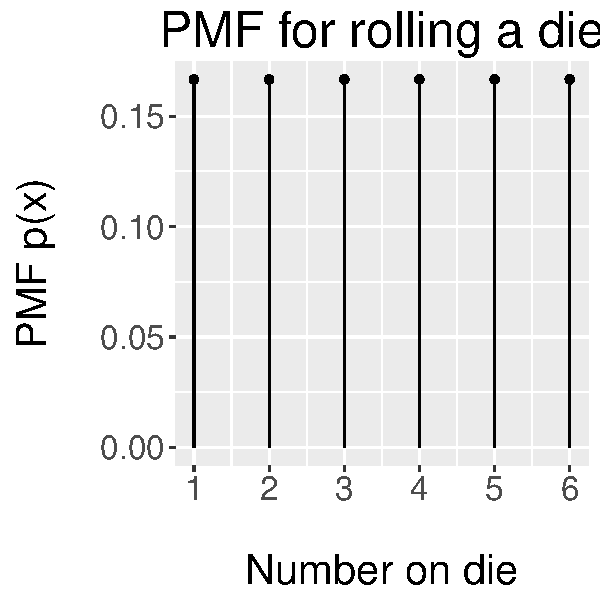
\includegraphics[scale=.4]{figures/DiePMF.pdf}\end{center}
\end{frame}

\begin{frame}[fragile]{How we made that PMF figure}
\begin{verbatim}
ggplot(data = data.frame(x = 1:6,
                         y = rep(1/6, 6),
                         yend = rep(0,6)),
       aes(x = x, y = y, xend = x, yend = yend)) +
  geom_point() +
  geom_segment() +
  scale_x_continuous(name="\nNumber on die", breaks=1:6) +
  scale_y_continuous(name="PMF p(x)\n") +
  ggtitle("PMF for rolling a die") +
  theme(text=element_text(size=20)) +
  ggsave("DiePMF.pdf",
         height=4,
         width=4)
\end{verbatim}
\end{frame}

\begin{frame}{When I roll a die, what is the CDF?}
$$P(X\leq 1)=1/6,\dots,P(X\leq 6)=6/6$$
$$P(X\leq x)=\begin{cases}
  0,& x<1 \\
  \lfloor x\rfloor/6,& x\in [1,6] \\
  1,& x>6
\end{cases}$$
\begin{center}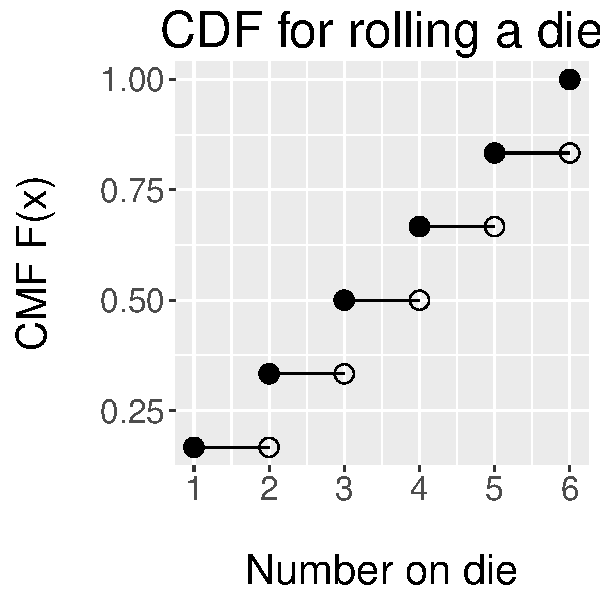
\includegraphics[scale=.4]{figures/DieCDF.pdf}\end{center}
\end{frame}
\begin{frame}[fragile]{How we made that CDF figure}
\begin{verbatim}
ggplot(data = data.frame(x = 1:6,
                         y = (1:6)/6,
                         xend = c(2:6,6))) +
  geom_point(aes(x = x, y = y), size = 4) +
  geom_segment(aes(x = x, xend = xend, y = y, yend = y)) +
  geom_point(aes(x = xend, y = y), shape = 1, size = 4) +
  scale_x_continuous(name="\nNumber on die",
                     breaks=1:6) +
  scale_y_continuous(name="CDF F(x)\n") +
  ggtitle("CDF for rolling a die") +
  theme(text=element_text(size=20)) +
  ggsave("DieCDF.pdf",
         height=4,
         width=4)
\end{verbatim}
\end{frame}

\begin{frame}{Which is a proper CDF? (check all that apply)}
\begin{center}

\includegraphics[scale=.4]{figures/Bullseye_Poll.png} \\
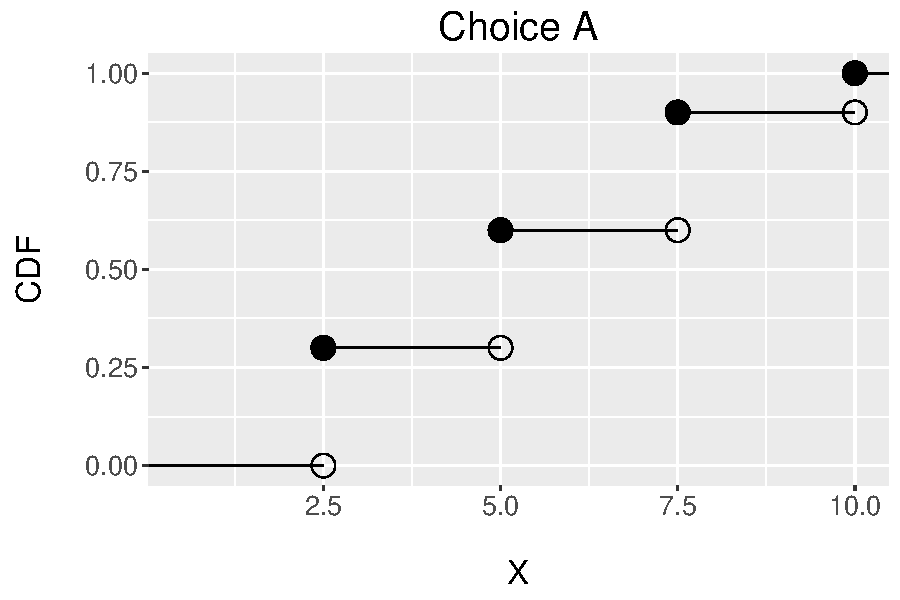
\includegraphics[scale=.32]{figures/CDF1.pdf}
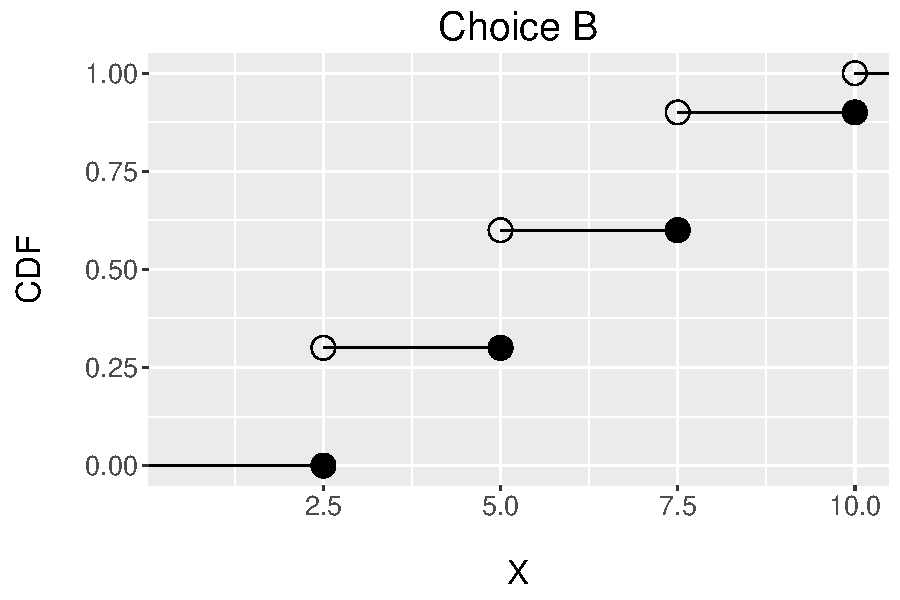
\includegraphics[scale=.32]{figures/CDF2.pdf} \\
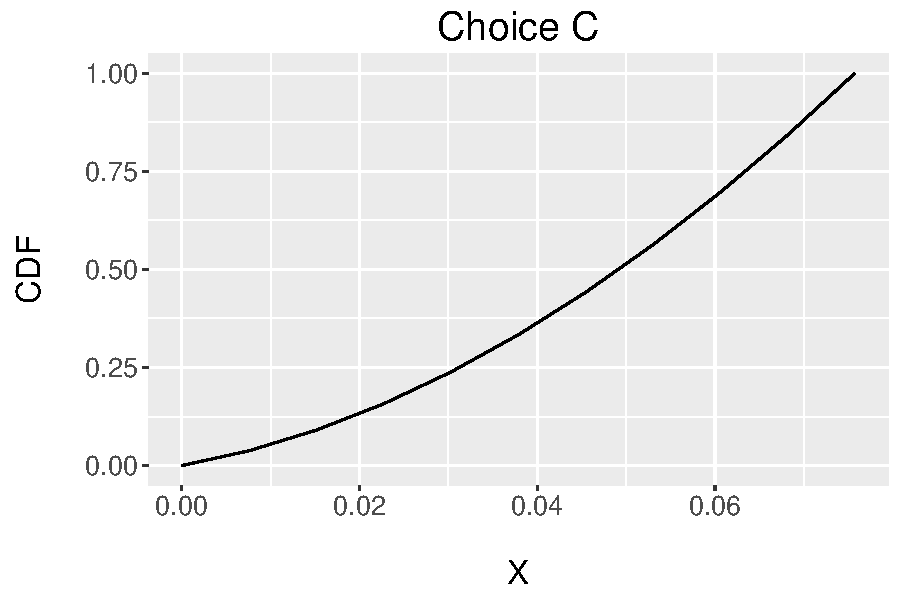
\includegraphics[scale=.32]{figures/CDF3.pdf}
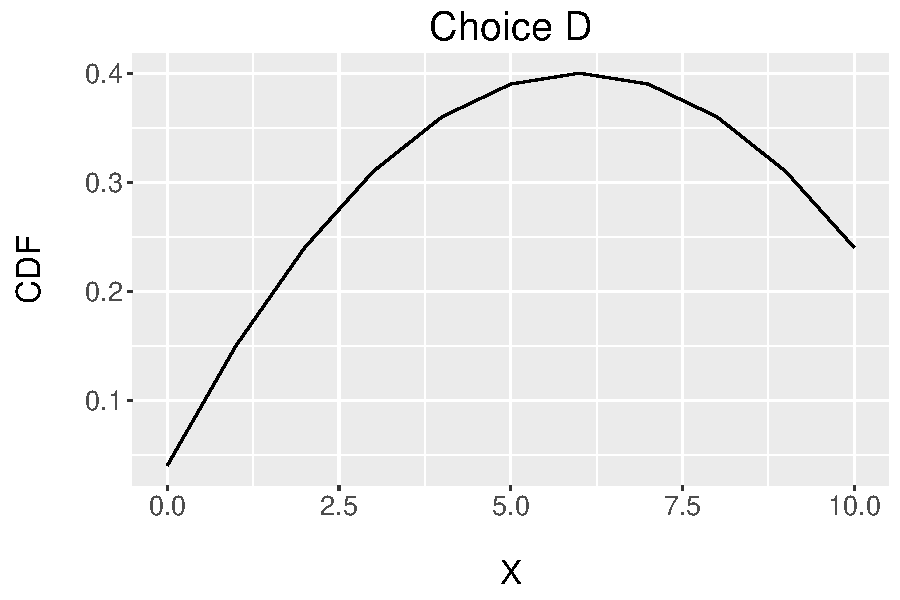
\includegraphics[scale=.32]{figures/CDF4.pdf}
\end{center}
\end{frame}

\begin{frame}{Properties of the CDF}
\begin{itemize}
\item Non-decreasing
\item Right continuous
\item $F(x)\rightarrow 0$ as $x\rightarrow -\infty$
\item $F(x)\rightarrow 1$ as $x\rightarrow \infty$
\end{itemize}
\end{frame}

\begin{frame}{Continuous random variables}

Suppose it is Lawnparties, and a very drunk Princetonian spins around ten times before throwing darts at a wall. Suppose the sides of the wall are marked 0 and 1. Ignoring the vertical position of the darts, the horizontal position of the darts might be distributed \alert{uniformly} over the interval.

$$U\sim Uniform(0,1)$$
The CDF of the uniform is
$$F(x)=x$$
\end{frame}

\begin{frame}
\centering
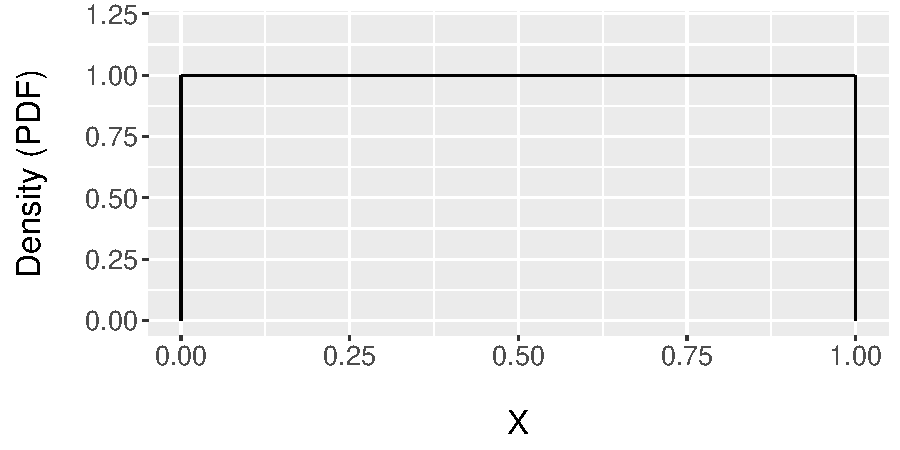
\includegraphics[scale=.5]{figures/Unif1a.pdf} \\
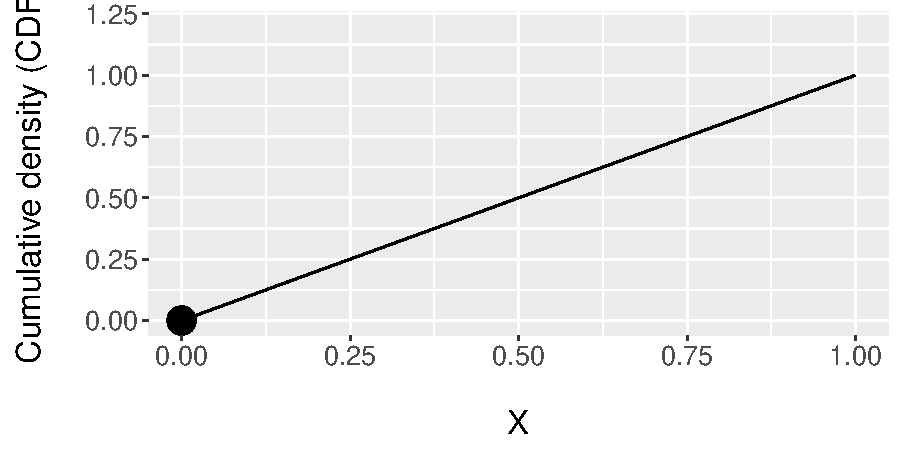
\includegraphics[scale=.5]{figures/Unif1b.pdf}
\end{frame}

\begin{frame}
\centering
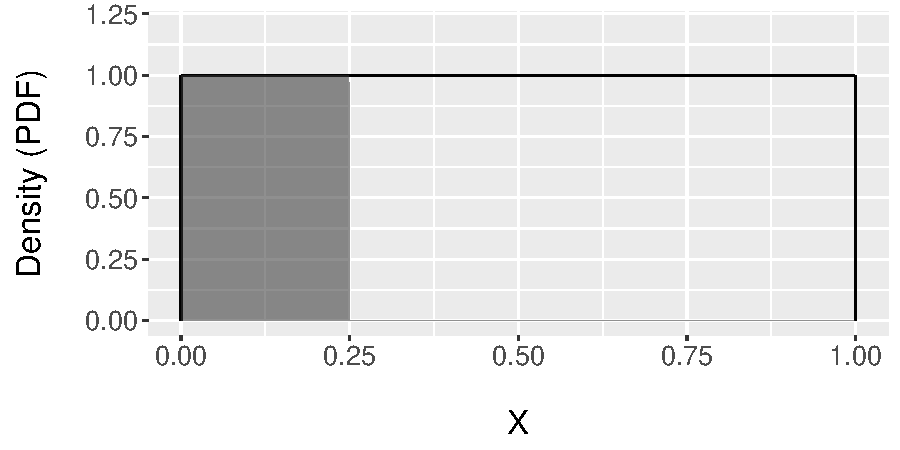
\includegraphics[scale=.5]{figures/Unif2a.pdf} \\
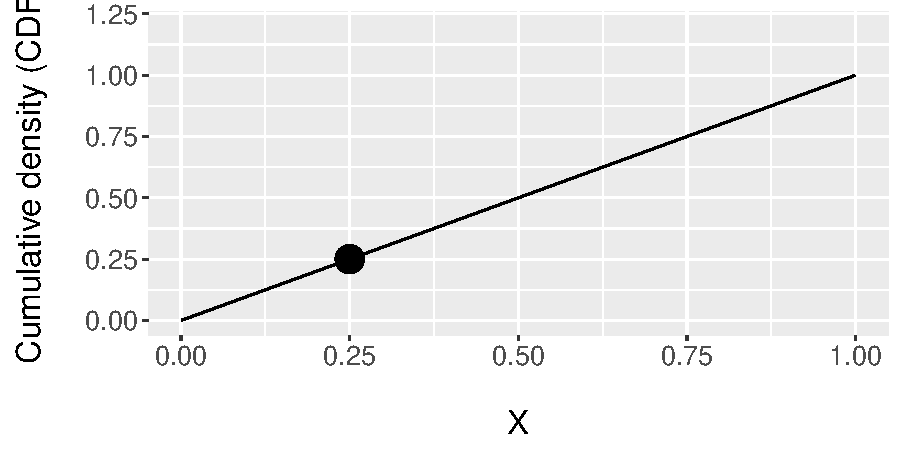
\includegraphics[scale=.5]{figures/Unif2b.pdf}
\end{frame}

\begin{frame}
\centering
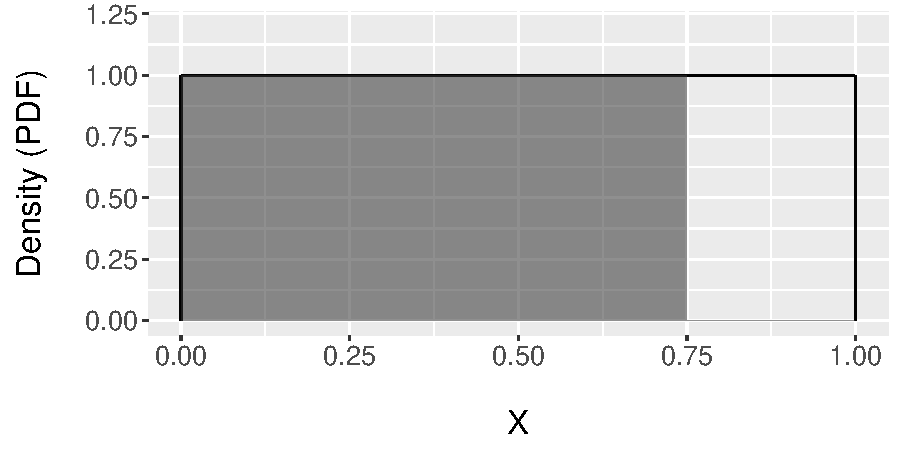
\includegraphics[scale=.5]{figures/Unif3a.pdf} \\
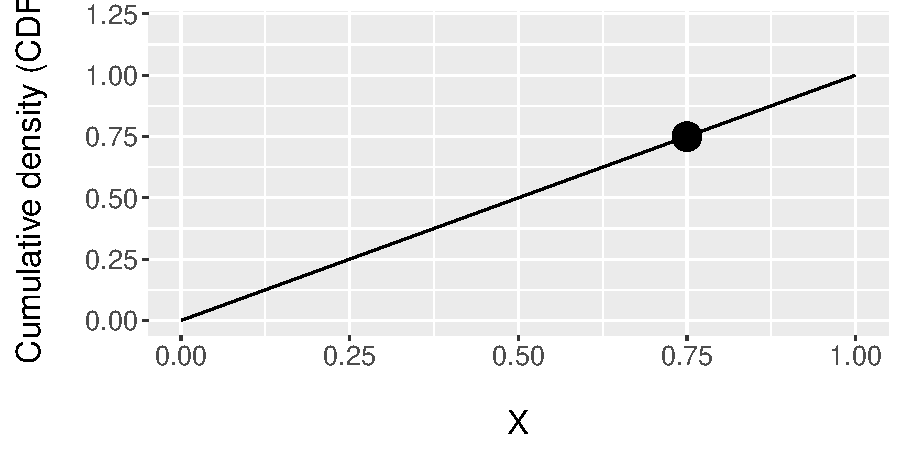
\includegraphics[scale=.5]{figures/Unif3b.pdf}
\end{frame}

\begin{frame}
\centering
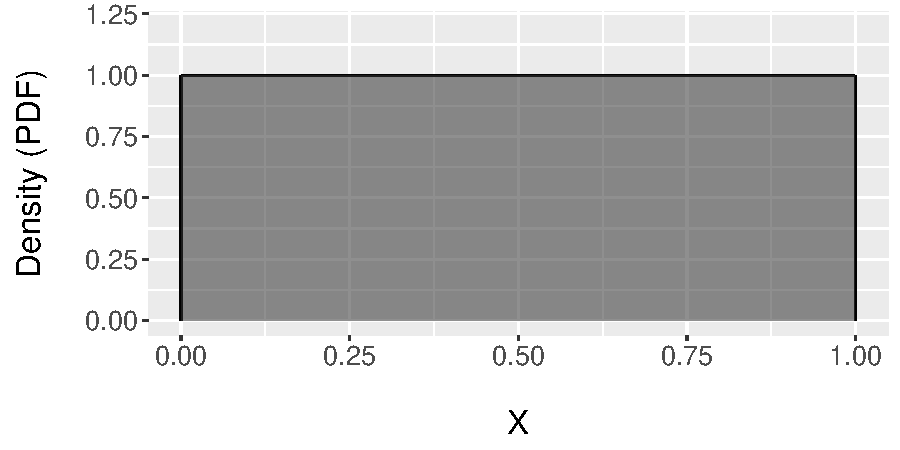
\includegraphics[scale=.5]{figures/Unif4a.pdf} \\
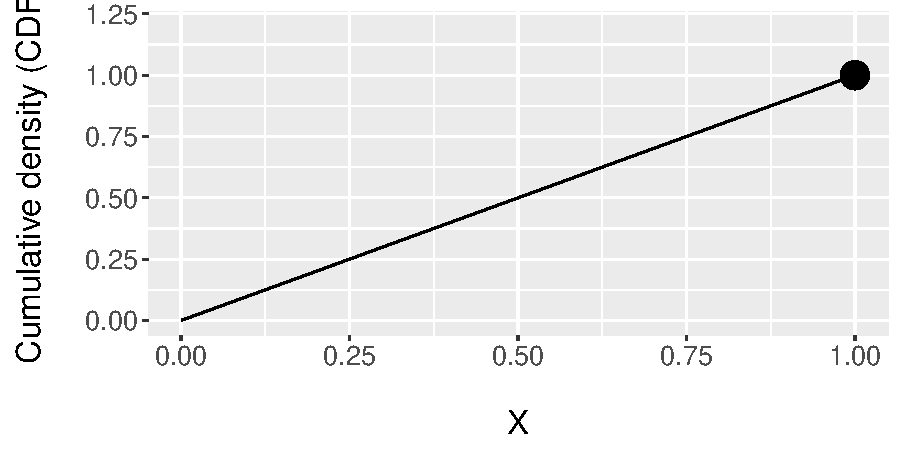
\includegraphics[scale=.5]{figures/Unif4b.pdf}
\end{frame}

\begin{frame}
What is the probability that a dart lands between 0.25 and 0.5?
\pause
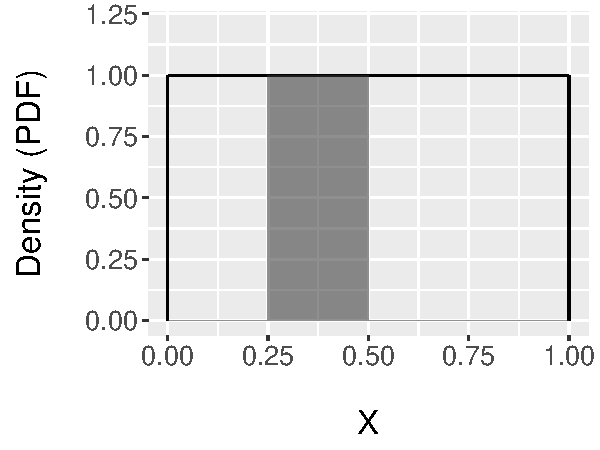
\includegraphics[scale=.5]{figures/Unif5a.pdf}
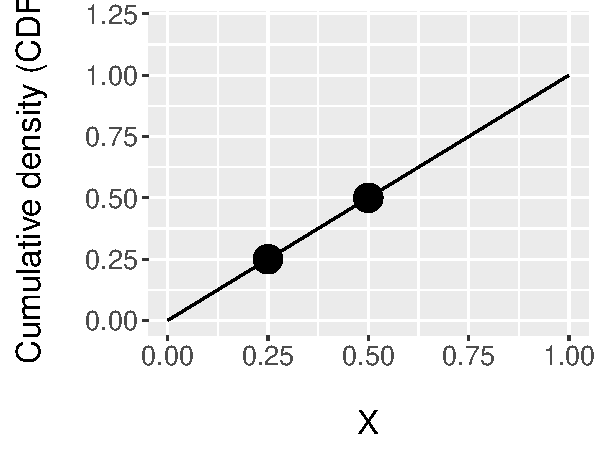
\includegraphics[scale=.5]{figures/Unif5b.pdf} \\
\pause
$$F(.5) - F(.25) = .25$$
\pause
The \texttt{punif()} command in \texttt{R} is the uniform cumulative distribution function:
\texttt{punif(.5) - punif(.25)}
\end{frame}

\begin{frame}

Now let's suppose we have someone better at throwing darts, so we're going to measure how far they are from the center of the wall in inches. In this case, perhaps the darts will be distributed \alert{normally} around the center of the wall.
$$X\sim N(\mu = 0, \sigma = 12)$$
\end{frame}

\begin{frame}
$$X\sim N(\mu = 0, \sigma = 12)$$
What is the probability of getting a bullseye ($X=0$)?
\\
\begin{center}
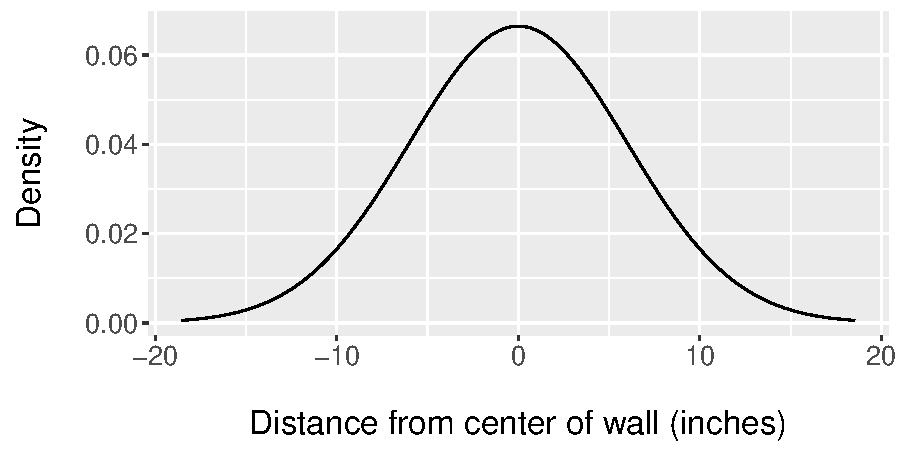
\includegraphics[scale=.5]{figures/Normal0.pdf} \\

\includegraphics[scale=.4]{figures/Bullseye_Poll.png}
\end{center}
\end{frame}

\begin{frame}
...we'll come back to that. \\
How would we calculate the probability that a dart lands within 6 inches of the center of the wall?
\pause
\begin{center}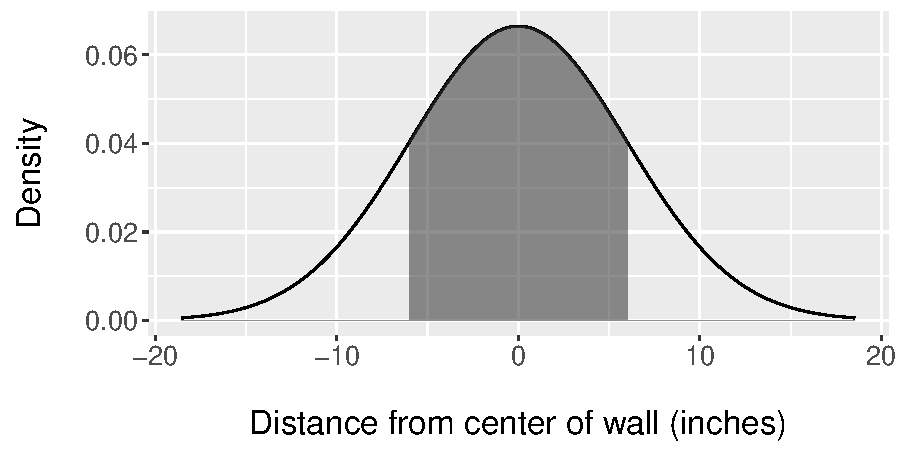
\includegraphics[scale=.6]{figures/Normal1.pdf}
\end{center}
\pause
$$P(X\in(-6,6)) = P(X<6)-P(X<-6) = \Phi(6) - \Phi(-6)$$
\pause
\begin{footnotesize}\texttt{pnorm(6, mean = 0, sd = 12) - pnorm(-6, mean = 0, sd = 12)}\end{footnotesize}
\end{frame}

\begin{frame}{One inch?}
\centering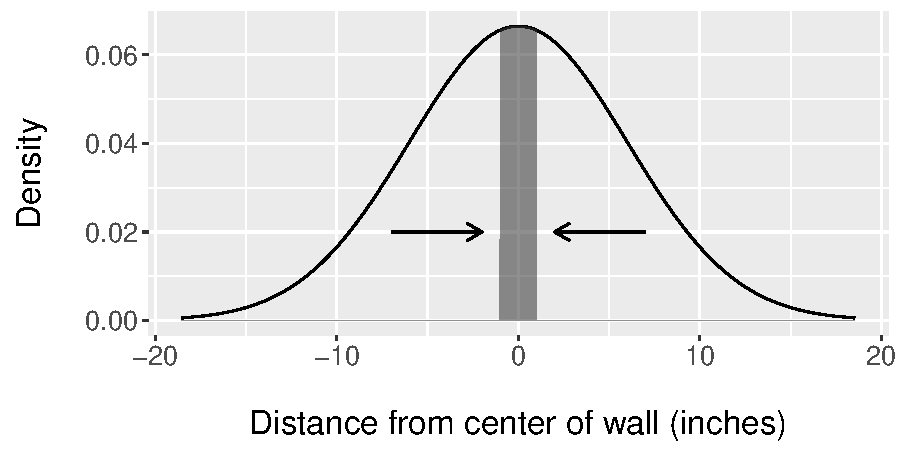
\includegraphics[scale=.6]{figures/Normal2.pdf}
\pause
$$P(X\in(-1, 1))=0.0664135$$
\end{frame}

\begin{frame}{1/100th of an inch?}
\centering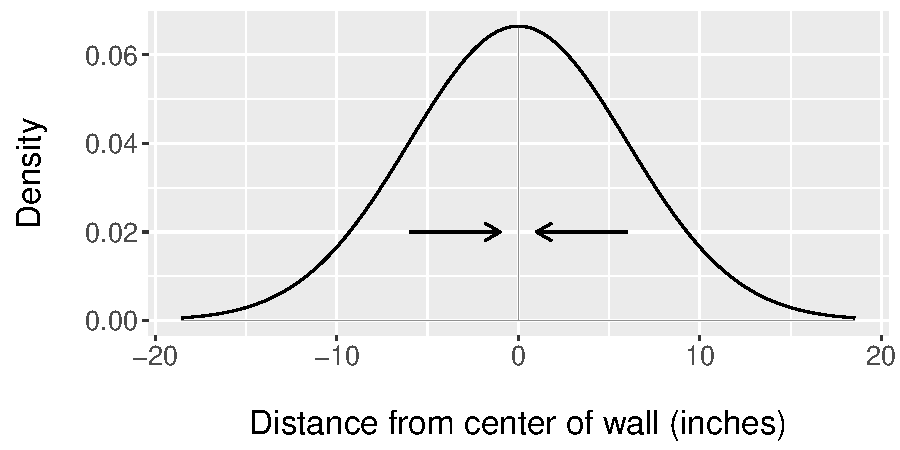
\includegraphics[scale=.6]{figures/Normal3.pdf}
\pause
$$P(X\in(-.01, .01))=0.0006649037$$
\end{frame}


\begin{frame}{A perfect bullseye?}
\centering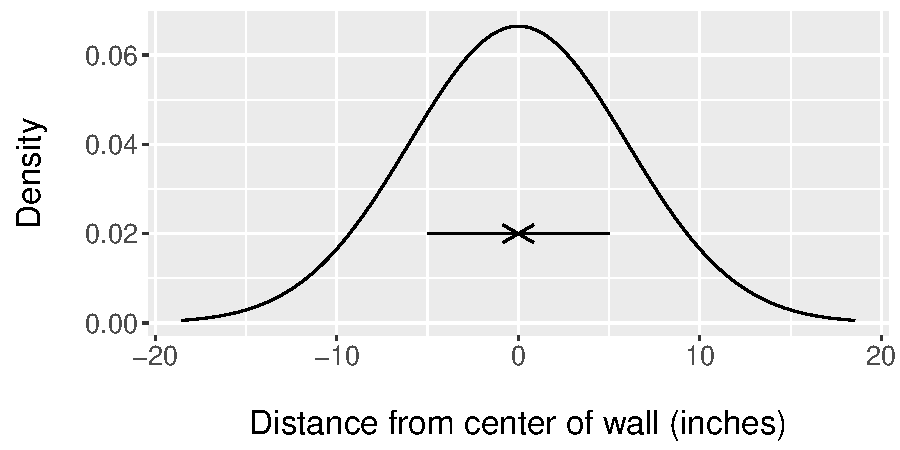
\includegraphics[scale=.6]{figures/Normal4.pdf}
\pause
$$P(X=0)=0$$
The probability that a continuous variable takes on any particular discrete value is \alert{0}!
\end{frame}

\begin{frame}{Useful R functions}
Let's type \texttt{?dnorm} into our R consoles. \pause \\
There are 4 functions for the normal distribution:
\begin{itemize}
\item \texttt{dnorm} gives the PDF
\item \texttt{pnorm} gives the CDF
\item \texttt{qnorm} is $F^{-1}()$: it gives quantiles
\item \texttt{rnorm} generates random draws
\end{itemize}
Question for the class: Can we recreate the \texttt{rnorm} using \texttt{qnorm} and \texttt{runif}?
\end{frame}

\begin{frame}{Universality of the Uniform}{aka Probability Integral Transform, PIT}
\begin{theorem}
\begin{footnotesize}
\begin{itemize}
\item Regardless of the distribution of $X$, $F(X)\sim Uniform(0,1)$
\item For a r.v. $X$ with CDF $F$ and a Uniform r.v. $U$, $F^{-1}(U)\sim X$
\end{itemize}
\end{footnotesize}
\end{theorem}
\begin{center}
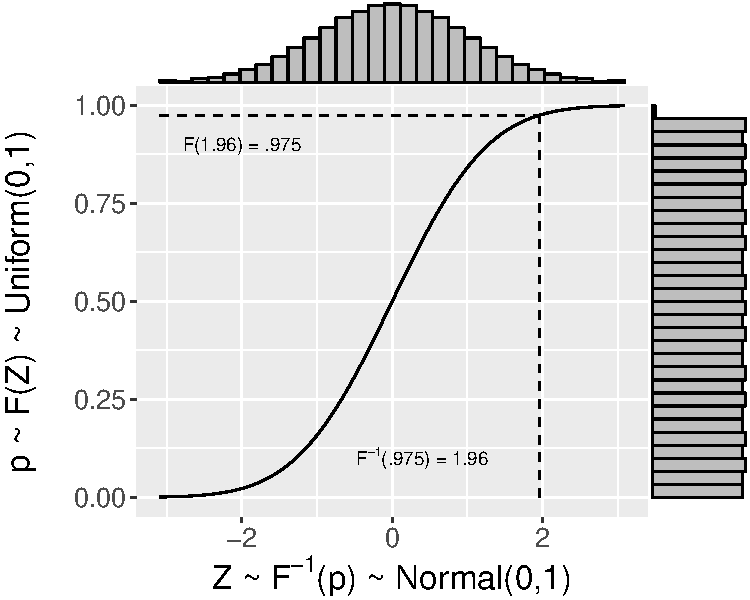
\includegraphics[scale=.55]{figures/UofU.pdf}
\end{center}
\end{frame}


\begin{frame}[fragile]{Self-written \texttt{rnorm}}

\begin{verbatim}
draw.rnorm <- function(n, mean = 0, sd = 1) {
  u <- runif(1)
  z <- qnorm(u)
  return(z)
}
qplot(x=draw.rnorm(1000), geom="histogram",
      bins = 30, xlim = c(-3,3))
qplot(x=rnorm(1000), geom="histogram",
      bins = 30, xlim=c(-3,3))
\end{verbatim}
\end{frame}

\begin{frame}{Did we succeed?}
\begin{center}
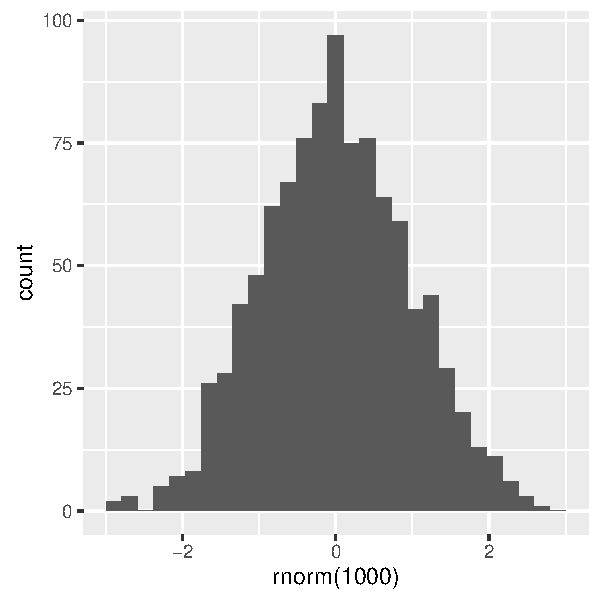
\includegraphics[scale=.5]{figures/rnorm_plot.pdf}
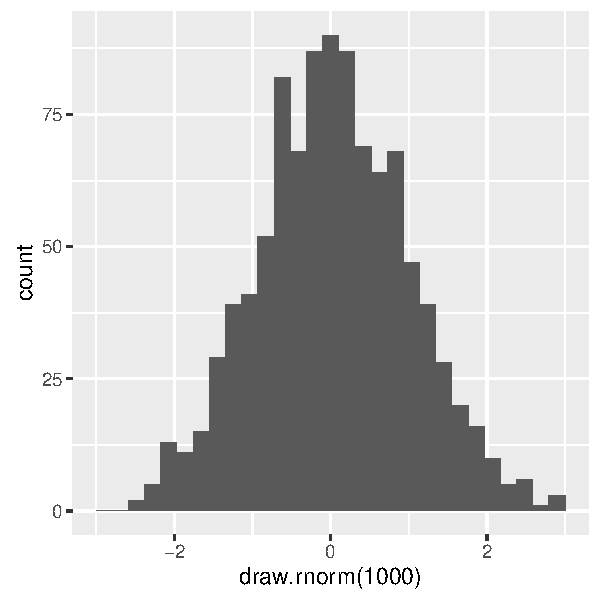
\includegraphics[scale=.5]{figures/draw_rnorm.pdf}
\end{center}
\end{frame}

\section{Expectation}
\begin{frame}{Definition of expectation}

$$E(X)=\begin{cases} \sum xp(x),& \text{if }X\text{ is discrete} \\
\int xf(x)dx,&\text{if }X\text{ is continuous}\end{cases}$$
\\
\alert{If you can write down the PDF or PMF, you can calculate the expected value.}
\end{frame}

\begin{frame}{Example: High jumpers}
Athletes compete one by one in a high jump competition. Let $X_j$ be how high the $j$th person jumped (in meters). Let $m$ be the median of the distribution of $X_j$. Let $N$ be the number of jumpers before the first one who successfully jumps higher than $m$ meters, not including that jumper. Find the mean of $N$.\\
\alert{What do we need?} \pause The PMF of $N$. \pause \\
\alert{What do we know?} \pause For each jumper $i$, $P(X_i<m)=\pause 0.5$ \\ \pause
\alert{Can we write down the PMF of $N$?} \\
\pause
$$P(N=0) = P(\text{first jumper clears}) = \pause 0.5$$
$$P(N=1) = P(\text{first jumper doesn't clear, and second does}) = \pause (0.5)0.5$$
$$P(N=2) = P(\text{first 2 jumpers don't clear, and third does}) = \pause (0.5^2)0.5$$
\end{frame}

\begin{frame}{High jumpers (continued)}
\begin{align*}
E(N) &= 0P(N=0) + 1P(N=1) + 2P(N=2) +... \\
&= 0(.5) + 1(.5).5 + 2(.5^2).5 +... \\
&= \sum_{x=0}^\infty x\left (.5^{x+1}\right ) \\
&= 1 \text{ by plugging in to WolframAlpha.com}
\end{align*}
The expected number of high jumpers to attempt before one clears the median jump height is 1.
\end{frame}

\begin{frame}{Linearity of Expectation: Questions}
Suppose $E(X)=\mu_x$ and $E(Y)=\mu_y$. Solve the following:
\begin{enumerate}
\item $E(X+Y) = $
\item $E(aX) = $
\item $E(aX+bY) = $
\item If $X$ and $Y$ are independent, what is $E\left(\frac{Y}{2}\mid X<4\right)$?
\end{enumerate}
\end{frame}

\begin{frame}{Linearity of Expectation: Answers}
Suppose $E(X)=\mu_x$ and $E(Y)=\mu_y$. Solve the following:
\begin{enumerate}
\item $E(X+Y) = E(X) + E(Y) = \mu_x+\mu_y$
\item $E(aX) = aE(X) = a\mu_x$
\item $E(aX+bY) = aE(X)+bE(Y) = a\mu_x + b\mu_y$
\item If $X$ and $Y$ are independent, what is $E\left(\frac{Y}{2}\mid X<4\right)$?
\end{enumerate}
Answer: $E(\frac{Y}{2}\mid X<4)=E\left(\frac{Y}{2}\right)\text{ (since independent) }=\frac{1}{2}E(Y)=\frac{\mu_y}{2}$
\end{frame}

\begin{frame}{Linearity of Expectation}
Suppose I flip a coin 20 times. What is the expected value of the number of heads? \\
\pause
for $i\in 1,\dots,20$,
$$X_i=\begin{cases}1,& \text{if heads} \\
0,& \text{if tails} \end{cases}$$
$$Y = (\#\text{ heads}) = X_1+X_2+...X_{20}$$
\pause
$$E(Y) = E\left (\sum_{i=1}^{20} X_i\right )$$
\pause
\begin{align*}
&=\sum_{i=1}^{20} E(X_i) \\
&=\sum_{i=1}^{20} 0.5 = 10
\end{align*}
\end{frame}

\begin{frame}{Law of Iterated Expectation (Adam's Law)}
\begin{theorem}
$$E(E[Y\mid X])=E(Y)$$
\end{theorem}
When calculating an expected value is hard, but would be easy if you knew something else, \alert{you can condition on that something else!}
\end{frame}

\begin{frame}{An example: Parking at the beach}
\centering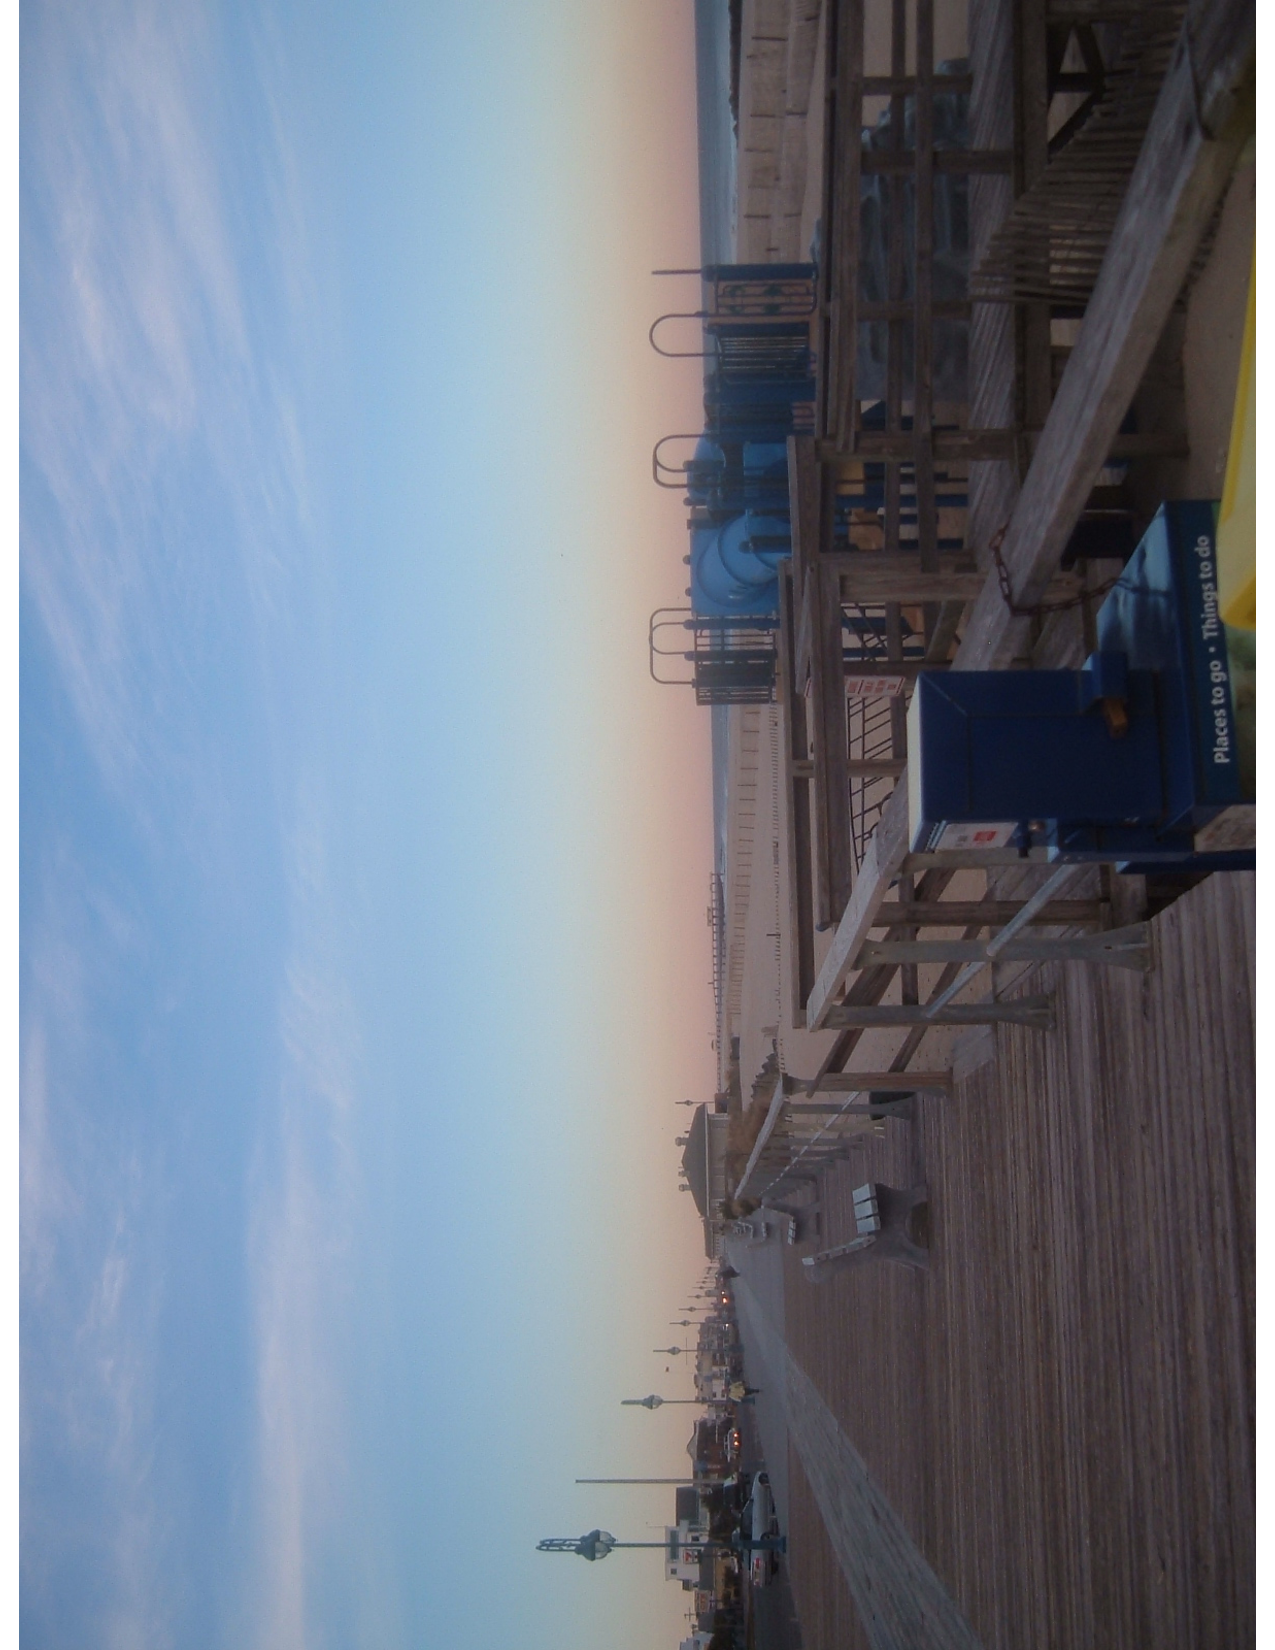
\includegraphics[angle=270,scale=.3]{figures/Belmar.pdf}
\end{frame}

\begin{frame}{Parking tickets at the beach}
Suppose you go to the beach in Belmar, NJ, and you park in the first row of spaces where there are meters, but you forget to pay the meter. Suppose the probability that you get a parking ticket (C for caught) is proportional to the time spent there (T), with the probability increasing log linearly with time
$$P(C \mid T) = \frac{1}{5}\left(T-\frac{1}{9}T^2\right)$$
Suppose the expected parking ticket is \$80 if you are caught, and when you go to the beach you stay 3 hours on average with a variance of 2 hours. What is your average parking ticket (F for fine) when you forget to pay the meter?
\end{frame}

\begin{frame}
\alert{What do we know?} $E(F\mid C)=80, P(C\mid T)=\frac{1}{5}\left(T-\frac{1}{9}T^2\right), E(T)=3, V(T)=2$ \\
\alert{What do we want?} $E(F)$ \\
$$E(F) = \pause E[E(F\mid C)] \pause = E[80C + 0(1-C)] = 80E(C)$$
\pause
$$E(C)=E(E[C\mid T])=E\left(\frac{1}{5}\left (T-\frac{1}{9}T^2\right)\right)$$
\pause
$$=\frac{1}{5}E(T)-\frac{1}{45}E(T^2)$$
\pause
$$V(T)=E(T^2)-[E(T)]^2 \rightarrow E(T^2)=V(T)+[E(T)]^2=2+3^2=11$$
\pause
$$E(C)=\frac{1}{5}(3)-\frac{1}{45}(11)=\frac{27}{45}$$
\pause
$$E(F)=80E(C)=80*\frac{16}{45}=\$28.44$$
\end{frame}

\begin{frame}{Real advice}
\centering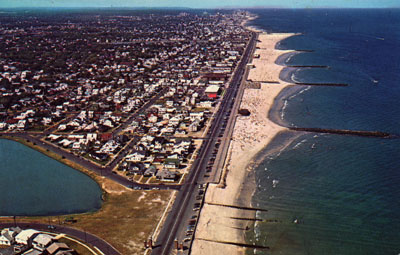
\includegraphics[scale=.5]{figures/Belmar_aerial.jpg}
\end{frame}

\section{Variance}
\begin{frame}{Variance is not a linear operator}
\begin{block}{Variance definition and rules}
$$V(X)=E(X-E[x])^2$$
$$V(X)=E(X^2)-(E[x])^2$$
$$V(aX+bY)=a^2V(X)+b^2V(Y)+2Cov(X,Y)$$
\end{block}
\begin{small}
Four problems: (assume $V(X)=\sigma^2_x$, $V(Y)=\sigma^2_y$, and $Cov(X,Y)=\rho$)
\begin{enumerate}
\item $V(5X) =$
\item $V(X+4) =$ 
\item $V(3X-2Y) = $
\item $V(X\mid X^2) = \text{assume for 4 that the distribution of }X\text{ is symmetric around 0}$
\end{enumerate}
\end{small}
\end{frame}

\begin{frame}{Law of Total Variance (Evve's Law)}
\begin{theorem}
$$V(Y)=E(V[Y\mid X])+V(E[Y\mid X])$$
\end{theorem}
\alert{Intuition:} Suppose $Y$ is income and $X$ is education. This says that the total variance in income can be divided into the expected amount of \alert{variance within categories} of education $E(V[Y\mid X])$ and the variance in expected incomes \alert{between categories} $V(E[Y\mid X])$.
\newline
\newline
We might think of $E(V[Y\mid X])$ as the variance in income that is not explained by education categories. More to come later in the semester!
\end{frame}

\begin{frame}
\begin{theorem}
$$V(Y)=E(V[Y\mid X])+V(E[Y\mid X])$$
\end{theorem}
Our fine example again (pun not intended): $F=$ fine, $C=$ whether caught.

$$V(F)=\pause E(V(F\mid C))+V(E(F\mid C))$$
\pause $$=E(0)+V(80C)$$
\pause $$=0+80^2V(C)$$
\pause
What is $V(C)$?
\pause
$$V(C)=E(V(C\mid T))+V(E(C\mid T))$$
This gets to ugly math, but you see the point. Conditioning makes the problem manageable!
\end{frame}

\begin{frame}{Poisson mean and variance in R: Useful for homework!}
A \textbf{Poisson} random variable
\begin{itemize}
\item captures counts of events
\item is parameterized by a rate of events, $\lambda$
\item both the mean and the variance are $\lambda$
\end{itemize}
\begin{center}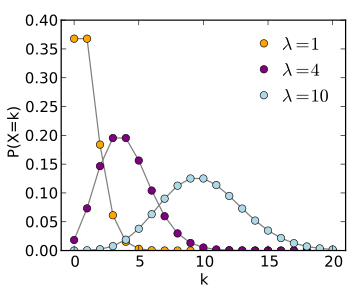
\includegraphics[scale=.3]{figures/PoissonPMF.png}\end{center}

Let's verify the mean and variance by simulation in \texttt{R}.
\end{frame}

\begin{frame}[fragile]{Poisson mean and variance in R: Useful for homework!}
\begin{footnotesize}
\begin{verbatim}
## Initialize Lambda vector
lambdas <- c(0.5, 1, 2)
## Initialize table to store results
pois_mean_var <- matrix(data = NA, nrow = 3, ncol = 2)
rownames(pois_mean_var) <- as.character(lambdas)
colnames(pois_mean_var) <- c("Mean", "Variance")
## Set a random seed
set.seed(08544)
for (lambda in lambdas) {
  pois_sim <- rpois(2000, lambda = lambda)
  ## Store simulated values in pois_mean_var
  pois_mean_var[as.character(lambda), ] <- 
    c(mean(pois_sim), var(pois_sim))
}
\end{verbatim}
\end{footnotesize}
\end{frame}

\begin{frame}[fragile]{Poisson example: Melting data}
\begin{footnotesize}
\begin{verbatim}
pois_mean_var
      Mean  Variance
0.5 0.4990 0.4992486
1   1.0315 1.0000078
2   1.9775 1.9659767
\end{verbatim}

We can use the \texttt{reshape2} package's \texttt{melt} function to change the shape of that data.
\begin{verbatim}
pois_mean_var_df <- melt(pois_mean_var)
   Var1     Var2     value
1   0.5     Mean 0.4990000
2   1.0     Mean 1.0315000
3   2.0     Mean 1.9775000
6   0.5 Variance 0.4992486
7   1.0 Variance 1.0000078
8   2.0 Variance 1.9659767
\end{verbatim}
\end{footnotesize}
\end{frame}

\begin{frame}[fragile]{Poisson example: easy ggplot()!}
\begin{footnotesize}
\begin{verbatim}
ggplot(pois_mean_var_df,
       aes(x = Var1,
           y = value,
           color = Var2)) +
  geom_point() +
  geom_line() +
  labs(title = "Means and Variances of Draws\n
                from the Poisson Distribution", 
       x = expression(~lambda), y = "Mean and Variance") +
  theme(legend.position = "bottom", legend.title=element_blank())
\end{verbatim}
\end{footnotesize}
\end{frame}

\begin{frame}{Poisson example: easy ggplot()!}
\begin{center}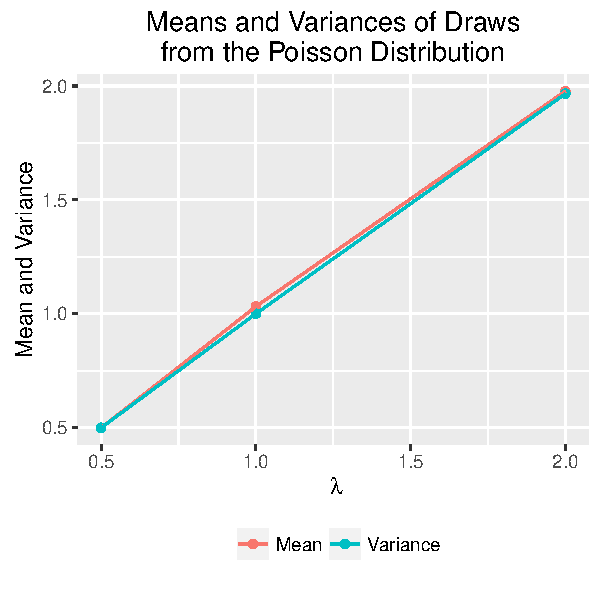
\includegraphics[scale=.8]{figures/MeltExample.pdf}\end{center}
\end{frame}

\begin{frame}{Covariance}
\begin{definition}
The \alert{covariance} of $X$ and $Y$ is defined as
$$Cov(X,Y)=E\left[(X-E[X])(Y-E[Y])\right]$$
\alert{Intuition:} If $X$ and $Y$ tend to be higher or lower than expected at the same time, then covariance is positive. \\
This formula can be simplified to this alternative:
$$Cov(X,Y)=E(XY)-E(X)E(Y)$$
\alert{Intuition:} Covariance is farther from 0 when it's more true that $E(XY)$ and $E(X)E(Y)$ give different things. Can we show that under independence the covariance is 0?
\end{definition}
\end{frame}

\begin{frame}{What Ian looks like at the start of a marthon}
\begin{center}
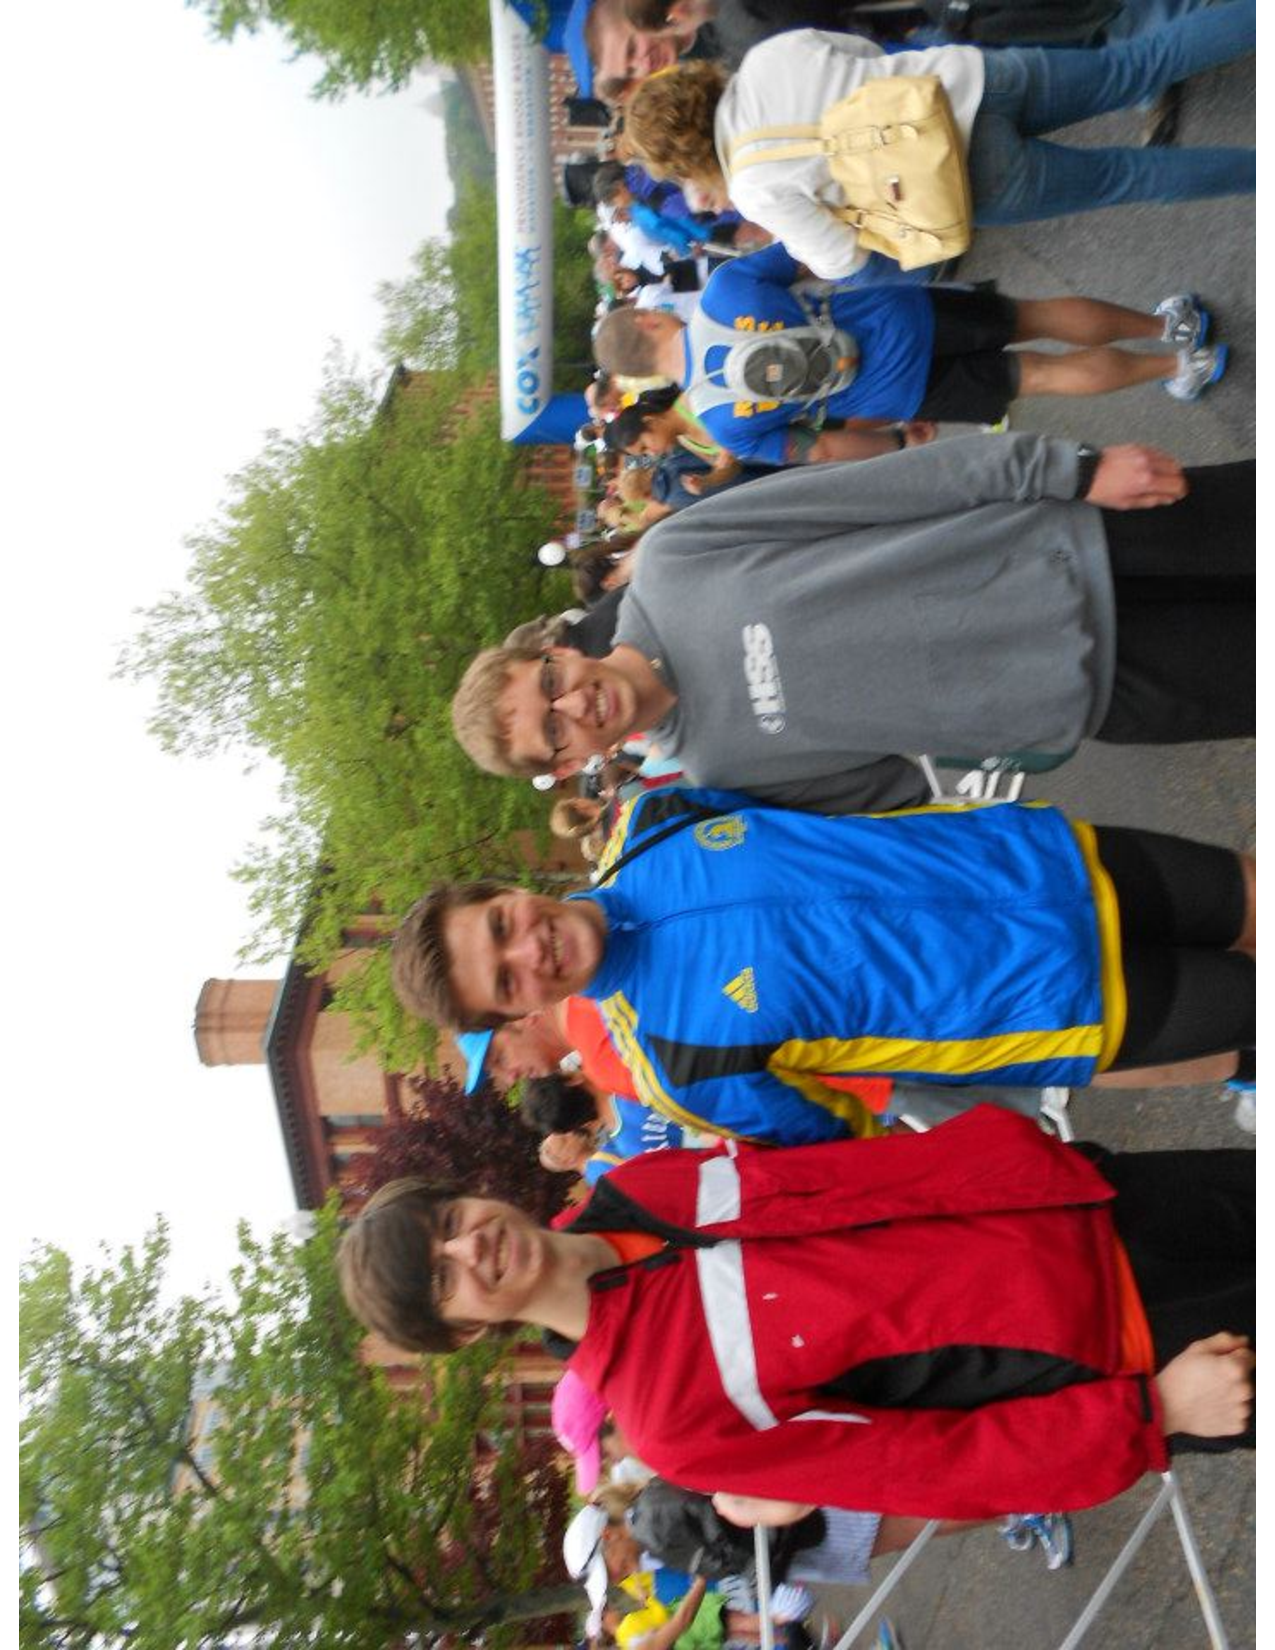
\includegraphics[angle=270,scale=.3]{figures/PreMarathon.pdf}
\end{center}
\end{frame}

\begin{frame}{...and 26.2 miles later}
\begin{center}
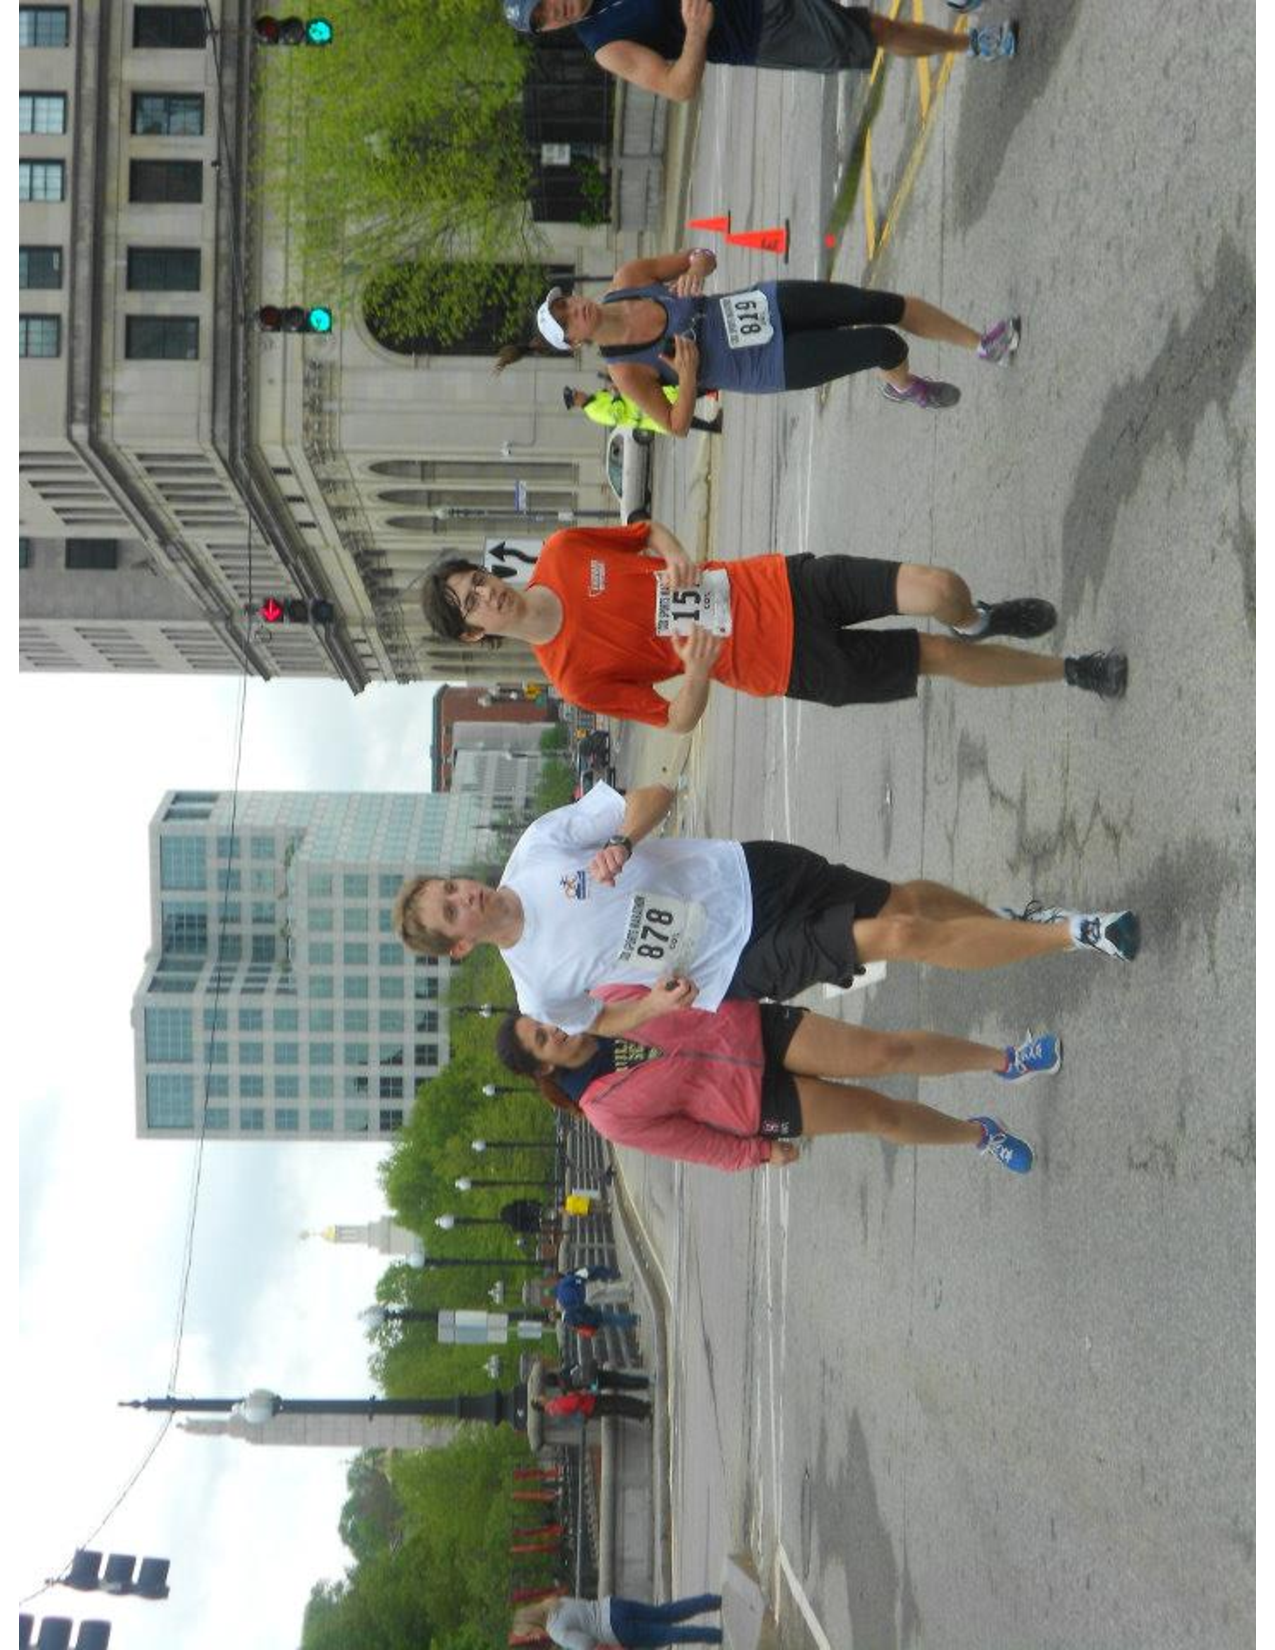
\includegraphics[angle=270,scale=.3]{figures/PostMarathon.pdf}
\end{center}
\end{frame}

\begin{frame}{Marathon times: Practice}
\begin{table}[ht]
\centering
\begin{tabular}{rccc}
 & \multicolumn{2}{c}{X: Time on first half (hrs)} \\
  \hline
Y: Time on second half (hrs) & 2 & 3 \\ 
  \hline
2 & 0.20 & 0.25 \\ 
  3 & 0.30 & 0.25 \\ 
   \hline
   \hline
\end{tabular}
\caption{Distribution of marathon times} 
\end{table}
\begin{enumerate}
\item Find $E(Y\mid X)$ for each possible $X$
\item Find $E(Y)$
\item Find $E(X)$
\item Find $E(XY)$
\item Find the covariance of $X$ and $Y$
\end{enumerate}
\end{frame}



\section{Benford's Law}
\begin{frame}\frametitle{Benford's Law\footnote{Benford's Law slides deeply indebted to Brandon Stewart and previous preceptors.}}
\begin{enumerate}
\item Law describing the (non-uniform) distribution of leading digits in many real-life sources of data.
\item Found in election results, populations of cities, stock market prices, word frequencies, death rates, street addresses and anything with a power law.
\item Often used for fraud detection.
\end{enumerate}
\end{frame}

\begin{frame}\frametitle{Benford's Law}
For base 10 counting systems, Benford's Law states that the leading digit has the probability distribution:
\begin{align*}
P(d) &= \text{log}_{10}(d + 1) - \text{log}_{10}(d) \\
&= \text{log}_{10}(1 + \frac{1}{d})
\end{align*}
Originally discovered by Simon Newcomb in 1881 but then restated and named after physicist Frank Benford in 1938.
\end{frame}

\begin{frame}\frametitle{Benford's Law}
\begin{figure}[h!]
\centering
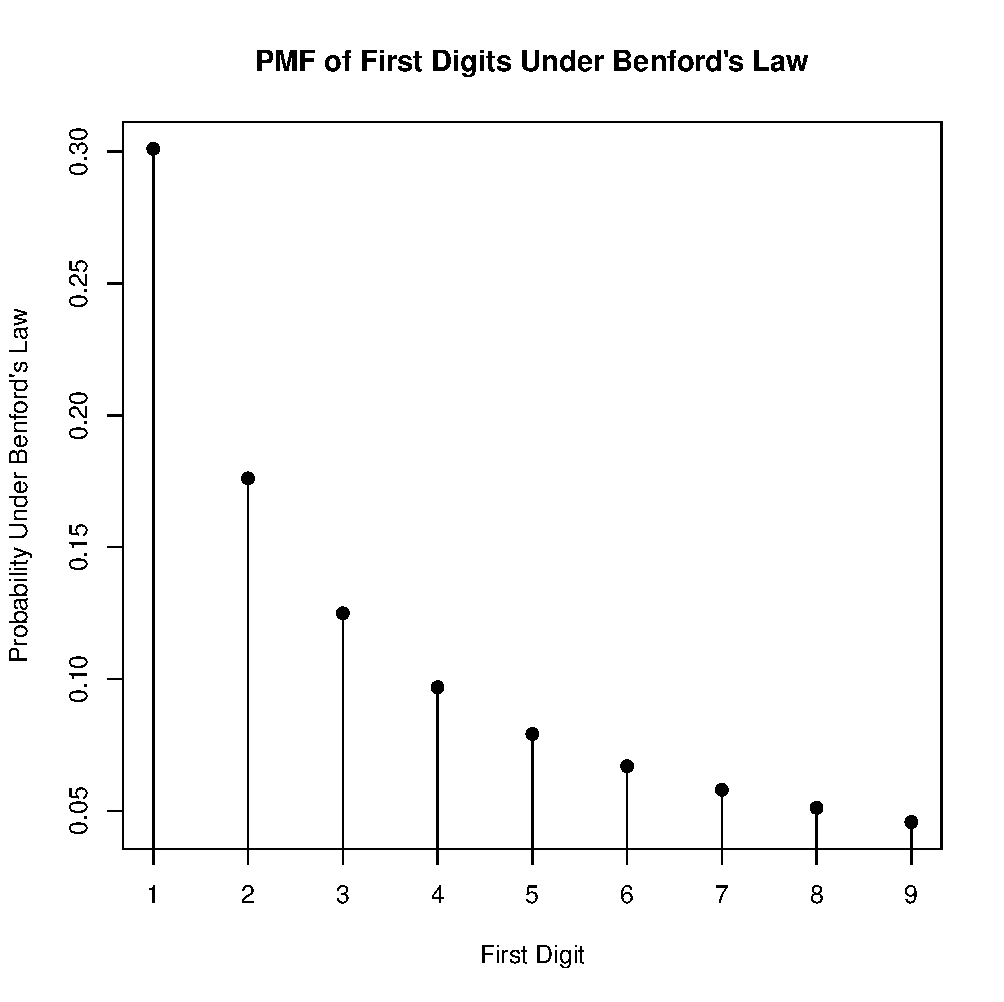
\includegraphics[scale=.4]{figures/Section2PMF.pdf}
\end{figure}
\end{frame}

\begin{frame}\frametitle{Benford's Law: Applications}
\begin{itemize}
\item Accounting Fraud (Nigrini, 1999)
\item Campaign Finance Fraud (Cho and Gaines, 2007)
\item Polling Fraud (Grebner and Weissman 2010)
\item Iranian Elections (Beber and Scacco 2009)
\end{itemize}
Benford's Law is admissible evidence of fraud in U.S. court!
\end{frame}

\begin{frame}\frametitle{Benford's Law: Data Rules\footnote{These come directly from Cho and Gaines (2007) formulation of the guidelines in Durtschi, Hillison and Pacini(2004)}}
Benford's Law works best under the following conditions:
\begin{itemize}
\item Numbers that result from combinations of other numbers (e.g. quantity times price)
\item Individual transactions like sales or data
\item Large datasets (these are asymptotic properties!)
\item Positive skew with mean greater than the median
\end{itemize}
It doesn't work as well in situations where:
\begin{itemize}
\item Numbers are assigned (check numbers, invoice numbers etc.)
\item There are procedural or psychological thresholds
\end{itemize}
Question: Why wouldn't this work with parking fines?
\end{frame}

\begin{frame}\frametitle{Benford's Law: Analytic Practice}
Let's practice our analytic skills by looking at the expectation and variance of first digits under Benford's Law: \\
How would we write the expectation of the first digit?
\begin{align*}
P(d) &= \text{log}_{10}(1 + \frac{1}{d})
\end{align*}
\end{frame}

\begin{frame}\frametitle{Benford's Law: Analytic Practice}
Let's practice our analytic skills by looking at the expectation and variance of first digits under Benford's Law: \\
How would we write the expectation of the first digit?
\begin{align*}
P(d) &= \text{log}_{10}(1 + \frac{1}{d}) \\
E(D) &= \sum_{i=1}^9 \text{log}_{10}(1 + \frac{1}{i})*i \\
&= 3.44 
\end{align*}
\end{frame}

\begin{frame}\frametitle{Benford's Law: Analytic Practice}
Let's practice our analytic skills by looking at the expectation and variance of first digits under Benford's Law: \\
How would we write the expectation of the first digit?
\begin{align*}
P(d) &= \text{log}_{10}(1 + \frac{1}{d}) \\
E(d) &= \sum_{i=1}^n \text{log}_{10}(1 + \frac{1}{i})*i \\
\end{align*}
How would you write the variance?
\end{frame}

\begin{frame}\frametitle{Benford's Law: Analytic Practice}
Let's practice our analytic skills by looking at the expectation and variance of first digits under Benford's Law: \\
How would we write the expectation of the first digit?
\begin{align*}
P(d) &= \text{log}_{10}(1 + \frac{1}{d}) \\
E(D) &= \sum_{i=1}^9 \text{log}_{10}(1 + \frac{1}{i})*i \\
&= 3.44 
\end{align*}
How would you write the variance?
\begin{align*}
V(D) &= \sum_{i=1}^9 \text{log}_{10}(1 + \frac{1}{i})(i - 3.44)^2  
\end{align*}
\end{frame}

\begin{frame}[fragile]{Benford's Law: Computational Practice}
Let's use \texttt{R} to generate the first 100 powers of 2
\pause
\begin{footnotesize}
\begin{verbatim} x <- sapply(0:100, function(x) 2^x) \end{verbatim}
\end{footnotesize}

Extract the leading digit from those
\pause
\begin{footnotesize}
\begin{verbatim}
extract.lead <- function(x.case) {
  lead <- as.numeric(strsplit(as.character(x.case),"")[[1]])[1]
}
leading <- sapply(x, extract.lead)
qplot(leading, geom="histogram", binwidth=1, alpha=.1)
\end{verbatim}
\end{footnotesize}
\end{frame}

\begin{frame}{Benford's Law: Computational Practice}
\begin{center}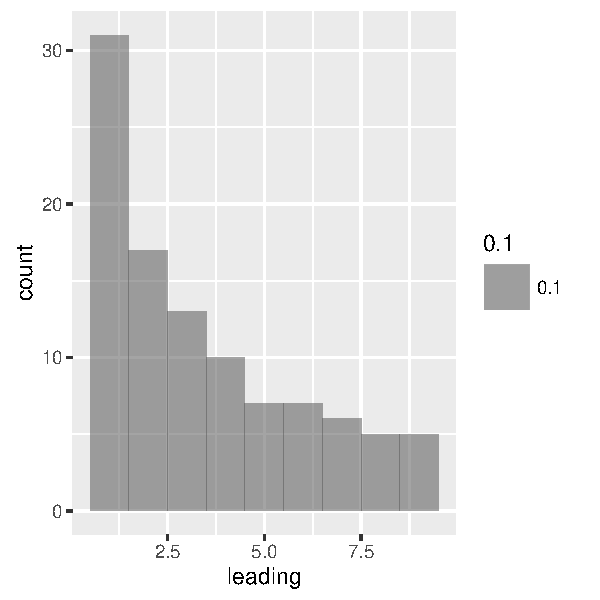
\includegraphics[scale=.7]{figures/Benford_powers_of_2.pdf}\end{center}
\end{frame}

\section{Joint Distributions}
\begin{frame}{Joint Distributions}
The joint distribution of $X$ and $Y$ is defined by a \alert{joint PDF} $f(x,y)$, or equivalently by a \alert{joint CDF} $F(x,y)$.

\begin{center}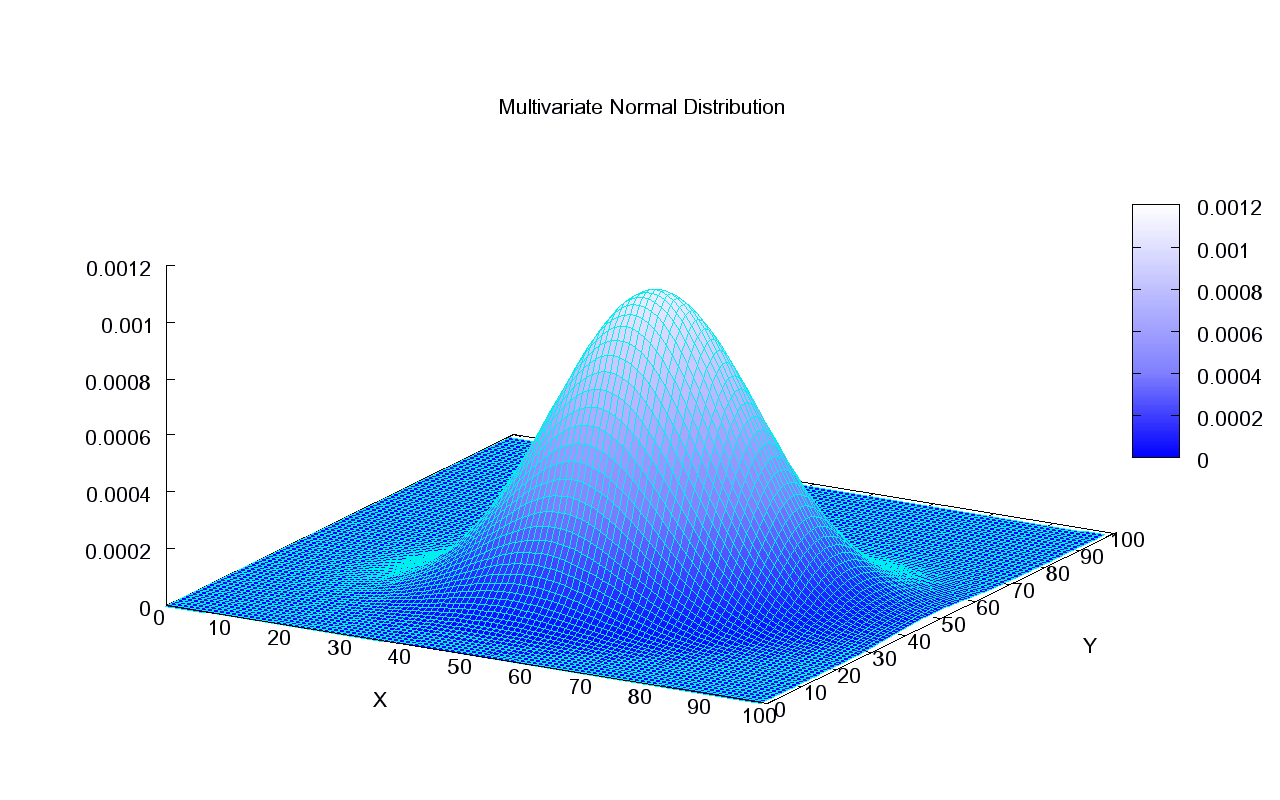
\includegraphics[scale=.2]{figures/Multivariate_Gaussian.png}\end{center}
\end{frame}

\begin{frame}{Join CDF visualization}
\begin{center}
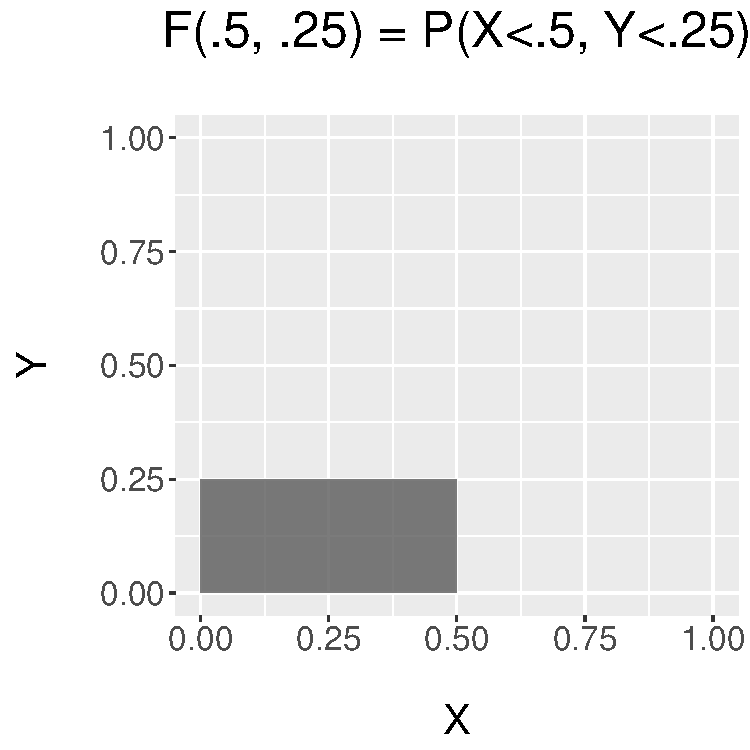
\includegraphics[scale=.6]{figures/Joint_CDF.pdf}
\end{center}
\end{frame}

\begin{frame}{CDF practice problem 1}{Modified from Blitzstein and Morris}

Suppose $a<b$, where $a$ and $b$ are constants (for concreteness, you could imagine $a=3$ and $b=5$). For some distribution with PDF $f$ and CDF $F$, which of the following must be true?
\begin{enumerate}
\item $f(a)<f(b)$
\item $F(a)<F(b)$
\item $F(a)\leq F(b)$
\end{enumerate}
\end{frame}

\begin{frame}{Joint CDF practice problem 2}{Modified from Blitzstein and Morris}

Suppose $a_1<b_1$ and $a_2<b_2$. Show that $F(b_1,b_2)-F(a_1,b_2)+F(b_1,a_2)-F(a_1,a_2)\geq 0$. \\
\pause
$$=\left[F(b_1,b_2)-F(a_1,b_2)\right]+\left[F(b_1,a_2)-F(a_1,a_2)\right]$$
\pause
$$=(\text{something }\geq 0) + (\text{something }\geq 0)$$
\pause
$$\geq 0$$
\end{frame}

\begin{frame}{Marginalizing}
\begin{center}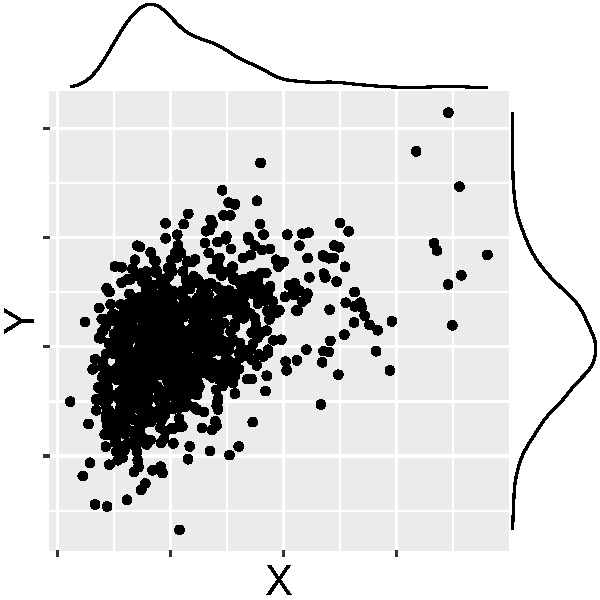
\includegraphics[scale=.7]{figures/Marginal_dists.pdf}\end{center}
\end{frame}

\section{Practice}

\begin{frame}{Correlation between sum and difference of dice}
\begin{small}
Suppose you roll two dice and get numbers $X$ and $Y$. What is $Cov(X+Y,X-Y)$?
\pause
\begin{block}{Note}
Covariance is a \alert{bilinear} operator, meaning that things distribute like multiplication.
$$Cov(aX,Y)=aCov(X,Y)$$
$$Cov(aX,bY)=abCov(X,Y)$$
$$Cov(X+Y,Z)=Cov(X,Z)+Cov(Y,Z)$$
\end{block}
\pause
$$Cov(X+Y,X-Y)=\pause Cov(X,X)-Cov(X,Y)+Cov(X,Y)-Cov(Y,Y)$$
\pause
$$=Var(X)-Var(Y)+Cov(X,Y)-Cov(X,Y)$$
\pause
$$=0 + 0 = 0$$
\end{small}
\end{frame}

\begin{frame}
Are $X+Y$ and $X-Y$ independent? Think of an extreme example.
\pause
\newline
\newline
Example: If $X+Y=2$, then $X=1$ and $Y=1$, so we know $X-Y=0$. Knowing $X+Y$ gives us some information about $X-Y$, so the two are not independent.
\end{frame}

\begin{frame}[fragile]{Sum and difference of dice: Simulation}
\pause
\begin{verbatim}
draw.sum.diff <- function() {
  x <- sample(1:6,1)
  y <- sample(1:6,1)
  return(c(x+y,x-y))
}
samples <- matrix(nrow=5000,ncol=2)
colnames(samples) <- c("x","y")
set.seed(08544)
for (i in 1:5000) {
  samples[i,] <- draw.sum.diff()
}
\end{verbatim}
\end{frame}

\begin{frame}[fragile]{Sum and difference of dice: Plot}
\pause
\begin{verbatim}
ggplot(data.frame(samples), aes(x=x,y=y)) +
  geom_point() +
  scale_x_continuous(breaks=c(2:12),
                     name="\nSum of dice") +
  scale_y_continuous(breaks=c(-5:5),
                     name="Difference of dice\n") +
  ggtitle("Sum and difference\nof two dice") +
  theme(text=element_text(size=20)) +
  ggsave("SumDiff.pdf",
         height=4, width=5)
\end{verbatim}
\end{frame}

\begin{frame}[fragile]{Sum and difference of dice: Plot}
\begin{center}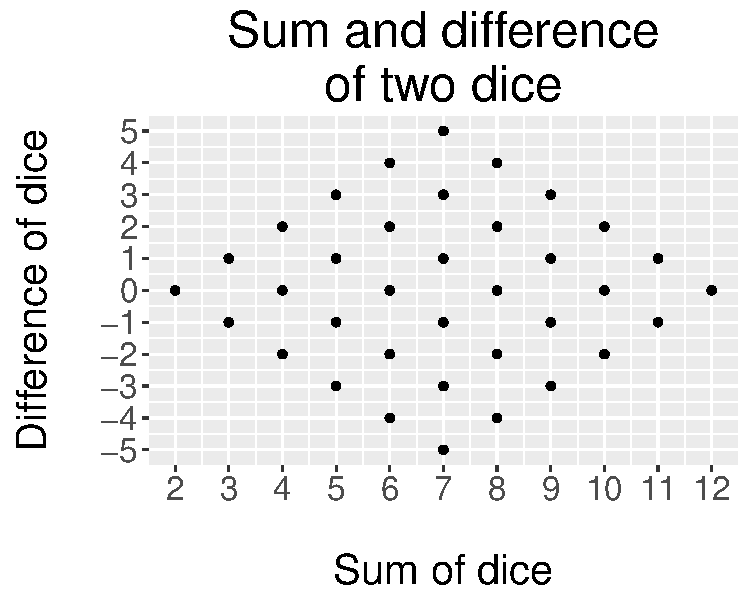
\includegraphics[scale=.7]{figures/SumDiff.pdf}\end{center}
\end{frame}

\begin{frame}{Examples to clarify independence}{Blitzstein and Hwang, Ch. 3 Exercises}
\begin{enumerate}
\item Give an example of dependent r.v.s $X$ and $Y$ such that $P(X<Y)=1$.
\item Can we have independent r.v.s $X$ and $Y$ such that $P(X<Y)=1$?
\item If $X$ and $Y$ are independent and $Y$ and $Z$ are independent, does this imply $X$ and $Z$ are independent?
\end{enumerate}
\end{frame}

\begin{frame}{Examples to clarify independence}{Blitzstein and Hwang, Ch. 3 Exercises}
\begin{enumerate}
\item Give an example of dependent r.v.s $X$ and $Y$ such that $P(X<Y)=1$.
\begin{itemize}
\item $Y\sim N(0,1)$, $X=Y-1$
\end{itemize}
\item Can we have independent r.v.s $X$ and $Y$ such that $P(X<Y)=1$?
\begin{itemize}
\item $X\sim Uniform(0,1)$, $Y\sim Uniform(2,3)$
\end{itemize}
\item If $X$ and $Y$ are independent and $Y$ and $Z$ are independent, does this imply $X$ and $Z$ are independent?
\begin{itemize}
\item No. Consider $X\sim N(0,1)$, $Y\sim N(0,1)$, with $X$ and $Y$ independent, and $Z=X$.
\end{itemize}
\end{enumerate}
\end{frame}

\begin{frame}{Measuring wealth}
\begin{footnotesize}Wealth inequality in America is dramatic and tightly coupled with race. The figure below shows estimated median net worth by race in 2005 and 2009, from a study by the Pew Research Center (\href{<http://citeseerx.ist.psu.edu/viewdoc/download?doi=10.1.1.397.5775&rep=rep1&type=pdf>}{link here}). The wealth distribution is also right-skewed (looks something like this simulated distribution).\end{footnotesize}
\newline
\newline
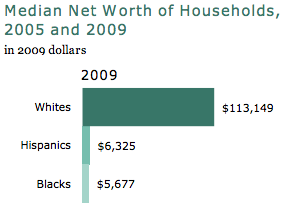
\includegraphics[scale=.5]{figures/Pew_wealth.png}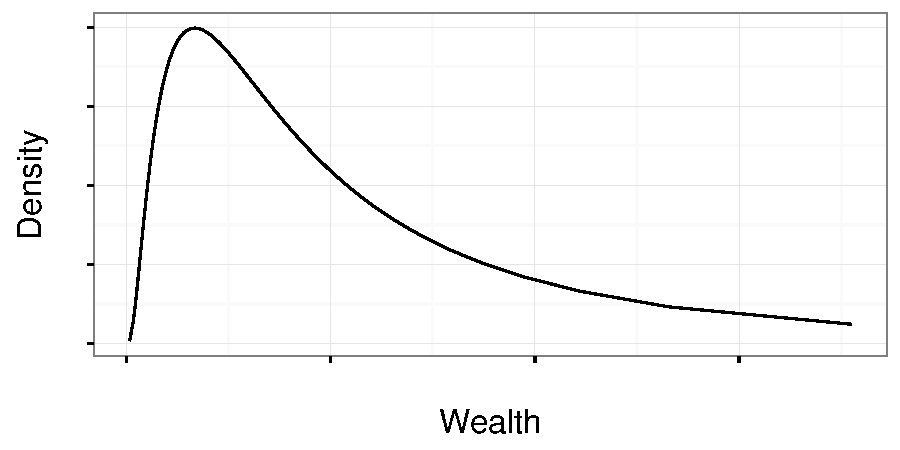
\includegraphics[scale=.3]{figures/WealthDist.pdf}

\alert{Question:} Would the mean of the wealth distribution be higher? Which report would you prefer?

\end{frame}

\begin{frame}{Wealth, part 2}
Suppose wealth is distributed log-normally, such that the log of wealth is normally distributed with mean 8.5 and standard deviation 1. Suppose a survey asks about wealth, but truncates responses above \$100,000. Can we find the expected report, both (a) analytically and (b) using \texttt{R}? Let $Y$ represent reported wealth and $Z$ represent true wealth.

Analytically: \pause
$$E(Y)=E(Y\mid Z<100,000)P(Z<100,000)$$
$$+E(Y\mid Z\geq 100,000)P(Z\geq 100,000)$$
\end{frame}

\begin{frame}{Wealth in R}
In \texttt{R}: \pause

\begin{alltt}
set.seed(08544) \\
z <- exp(rnorm(n = 10000, mean = 8.5, sd = 1)) \\
y <- z \\
y[y>=100000] <- 100000 \\
mean(z) \\
mean(y) \\
\end{alltt}

How does median wealth compare to the mean? \\
\texttt{median(z)}
\end{frame}

\begin{frame}{The power of conditioning: Coins}
Suppose your friend has two coins, one which is fair and one which has a probability of heads of 3/4. Your friend picks a coin randomly and flips it. What is the probability of heads?
\pause
$$P(H)=\pause P(H\mid F)P(F)+P(H\mid F^C)P(F^C)$$
\pause
$$=0.5(.05)+.75(.05)=0.625$$
\pause
Suppose the flip was heads. What is the probability that the coin chosen was fair?
$$P(F\mid H)=\pause\frac{P(H\mid F)P(F)}{P(H)}$$
\pause
$$=\frac{0.5(0.5)}{0.625)}=0.4$$
\end{frame}

\section{Representation}
\begin{frame}{Exponential: $-\log$ Uniform}{Figure credit: Wikipedia}
The Uniform distribution is defined on the interval $(0,1)$. Suppose we wanted a distribution defined on all positive numbers.
\begin{definition}
$X$ follows an \textbf{exponential} distribution with rate parameter $\lambda$ if
$$X\sim -\frac{1}{\lambda} log(U)$$
\end{definition}
\begin{center}\includegraphics[scale=.3]{figures/ExpoPDF.png}\end{center}
\end{frame}

\begin{frame}{Exponential: $-\log$ Uniform}
The exponential is often used for wait times. For instance, if you're waiting for shooting stars, the time until a star comes might be exponentially distributed.

Key properties:
\begin{itemize}
\item Memorylessness: Expected remaining wait time does not depend on the time that has passed
\item $E(X)=\frac{1}{\lambda}$
\item $V(X)=\frac{1}{\lambda^2}$
\end{itemize}
\end{frame}

\begin{frame}{Exponential-uniform connection}
Suppose $X_1,X_2\stackrel{iid}{\sim} Expo(\lambda)$. What is the distribution of $\frac{X_1}{X_1+X_2}$?
\pause
The proportion of the wait time that is represented by $X_1$ is uniformly distributed over the interval, so
$$\frac{X_1}{X_1+X_2}\sim Uniform(0,1)$$
\end{frame}

\begin{frame}{Gamma: Sum of independent Exponentials}{Figure credit: Wikipedia}
\begin{definition}
Suppose we are waiting for $a$ shooting stars, with the time between stars $X_1,\dots,X_a\stackrel{iid}{\sim}Expo(\lambda)$. The distribution of time until the $a$th shooting star is
$$G\sim \sum_{i=1}^a X_i\sim Gamma(a,\lambda)$$
\end{definition}
\begin{center}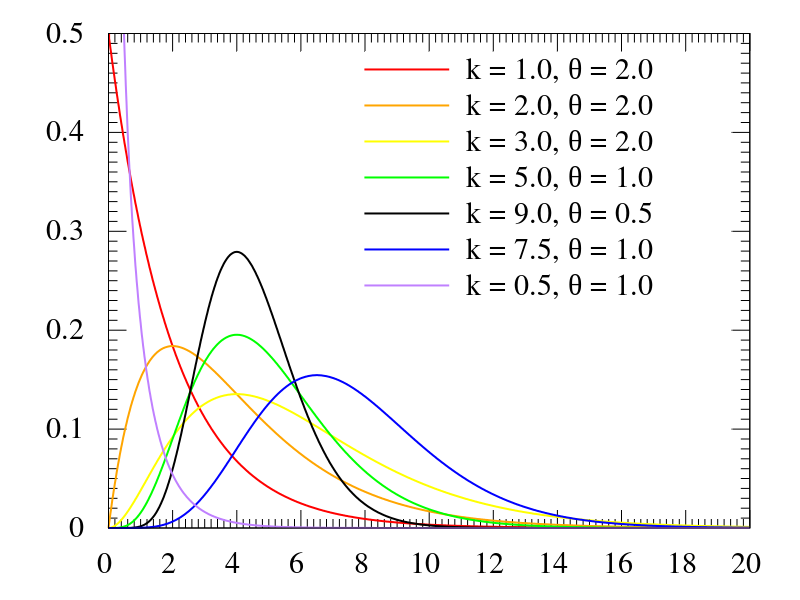
\includegraphics[scale=.15]{figures/GammaPDF.png}\end{center}
\end{frame}

\begin{frame}{Gamma: Properties}
Properties of the $Gamma(a,\lambda)$ distribution include:
\begin{itemize}
\item $E(G)=\frac{a}{\lambda}$
\item $V(G)=\frac{a}{\lambda^2}$
\end{itemize}
\end{frame}

\begin{frame}{Beta: Uniform order statistics}
Suppose we draw $U_1,\dots,U_k\sim Uniform(0,1)$, and we want to know the distribution of the $j$th \emph{order statistic}, $U_{(j)}$. Using the Uniform-Exponential connection, we could also think of these $U_{(j)}$ as being the location of the $j$th Exponential in a series of $k+1$ Exponentials. Thus,
$$U_{(j)}\sim \frac{\sum_{i=1}^j X_i}{\sum_{i=1}^{j} X_i+\sum_{i=j+1}^{k+1} X_i}\sim Beta(j,k-j+1)$$
This defines the \textbf{Beta distribution}.

Can we name the distribution at the top of the fraction?
\pause
$$\sim \frac{G_j}{G_j+G_{k-j+1}}$$
\end{frame}

\begin{frame}{What do Betas look like?}{Figure credit: Wikipedia}
\begin{center}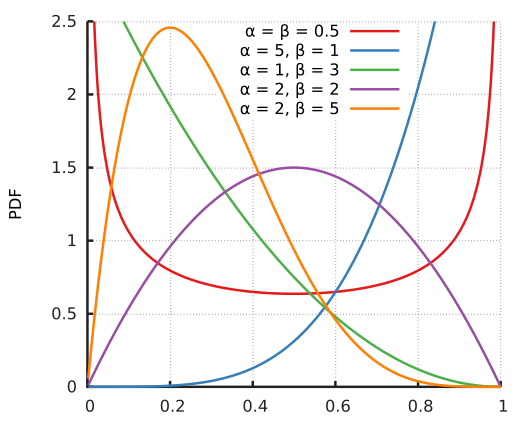
\includegraphics[scale=.3]{figures/BetaPDF.png}\end{center}
\end{frame}

\begin{frame}{Poisson: Number of Exponential events in a time interval}{Figure credit: Wikipedia}
\begin{definition}
Suppose the time between shooting stars is distributed $X\sim Expo(\lambda)$. Then, the number of shooting stars in an interval of time $t$ is distributed
$$Y_t\sim Poisson(\lambda t)$$
\end{definition}
\begin{center}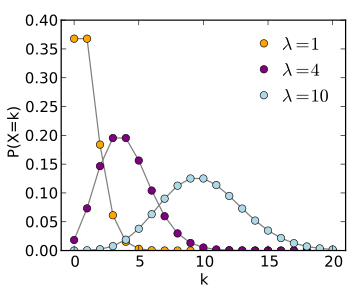
\includegraphics[scale=.3]{figures/PoissonPMF.png}\end{center}
\end{frame}

\begin{frame}{Poisson: Number of Exponential events in a time interval}
Properties of the Poisson:
\begin{itemize}
\item If $Y\sim Pois(\lambda t)$, then $V(Y)=E(Y)=\lambda t$
\item Number of events in disjoint intervals are independent
\end{itemize}
\end{frame}

\begin{frame}{$\chi^2_n$: A particular Gamma}
\begin{definition}
We define the \textbf{chi-squared distribution} with $n$ degrees of freedom as
$$\chi^2_n\sim Gamma\left(\frac{n}{2},\frac{1}{2}\right)$$
\end{definition}
More commonly, we think of it as the sum of a series of independent squared Normals, $Z_1,\dots,Z_n\stackrel{iid}{\sim}Normal(0,1)$:
$$\chi^2_n\sim \sum_{i=1}^n Z_i^2$$
\end{frame}

\begin{frame}{$\chi^2_n$: A particular Gamma}{Figure credit: Wikipedia}
\begin{center}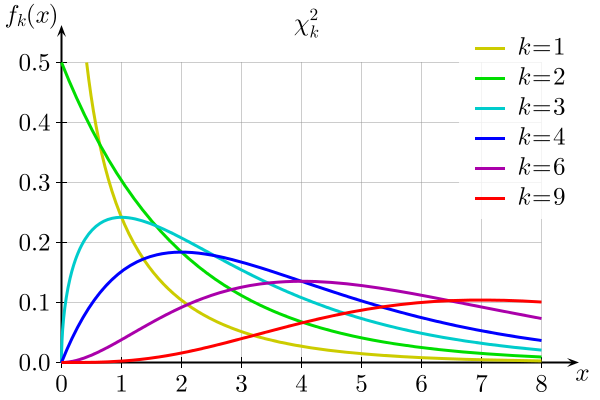
\includegraphics[scale=.4]{figures/Chi2PDF.png}\end{center}
\end{frame}

\begin{frame}{Normal: Square root of $\chi^2_1$ with a random sign}{Figure credit: Wikipedia}
\begin{definition}
$Z$ follows a \textbf{Normal} distribution if $Z\sim S\sqrt{\chi^2_1}$, where $S$ is a random sign with equal probability of being 1 or -1.
\end{definition}
\begin{center}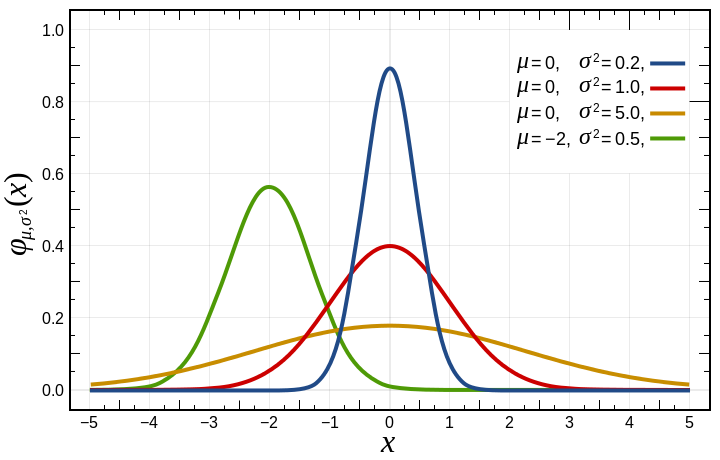
\includegraphics[scale=.3]{figures/NormalPDF.png}\end{center}
\end{frame}


\begin{frame}{Normal: An alternate construction}{Note: This is far above and beyond what you need to understand for the course!}
\begin{block}{Box-Muller Representation of the Normal}
Let $U_1,U_2\stackrel{iid}{\sim}Uniform$. Then
$$Z_1\equiv \sqrt{-2 \log U_2}\cos(2\pi U_1)$$
$$Z_2\equiv \sqrt{-2 \log U_2}\sin(2\pi U_1)$$
so that $Z_1,Z_2\stackrel{iid}{\sim} N(0,1)$
\end{block}
\begin{footnotesize}
What is this?
\begin{itemize}
\item \textbf{Inside the square root:} $-2\log U_2\sim Expo\left(\frac{1}{2}\right)\sim Gamma\left(\frac{2}{2},\frac{1}{2}\right)\sim \chi^2_2$
\item \textbf{Inside the cosine and sine:} $2\pi U_1$ is a uniformly distributed angle in polar coordinates, and the $\cos$ and $\sin$ convert this to the cartesian $x$ and $y$ components, respectively.
\item \textbf{Altogether in polar coordinates:} The square root part is like a radius distributed $\chi\sim |Z|$, and the second part is an angle.
\end{itemize}
\end{footnotesize}
\end{frame}

\begin{frame}{Key formulas we reviewed}
\begin{footnotesize}
CDF: $F_X(x)=P(X<x)$ \\
\medskip
PDF: $f_X(x)=\frac{\partial}{\partial x}F_X(x)$ (this $\neq P(X=x)$, which is 0!) \\
\medskip
Definition of expectation: $E(X)=\begin{cases}\sum_x xp(x),& \text{ if }x\text{ discrete} \\
\int x f(x) dx,&\text{ if }x\text{ continuous}\end{cases}$ \\
\medskip
LOTUS (Law of the Unconscious Statistician):
$$E(g[X])=\begin{cases}\sum_x g(x)p(x),& \text{ if }x\text{ discrete} \\
\int g(x) f(x) dx,&\text{ if }x\text{ continuous}\end{cases}$$ \\
\medskip
Adam's law (iterated expectation): $E(Y)=E(E[Y\mid X])$ \\
\medskip
Evve's law (total variance): $V(Y)=E(V[Y\mid X])+V(E[Y\mid X])$
\end{footnotesize}
\end{frame}

\begin{frame}{Key formulas we reviewed}
\begin{footnotesize}
Variance of sums:
$$V(aX+bY)=a^2X+b^2Y+2abCov(X,Y)$$
$$V(aX-bY)=a^2x+b^2Y-2abCov(X,Y)$$
\medskip
Definition of variance:
\begin{align*}
V(X)&=E\left[\left(X-E[X]\right)^2\right] \\
&=E\left(X^2-\left[E(X)\right]^2\right)
\end{align*}
\medskip
Definition of covariance:
\begin{align*}
Cov(X,Y)&=E\left[\left(X-E[X]\right)\left(Y-E[Y]\right)\right] \\
&=E\left(XY-E[X]E[Y]\right)
\end{align*} \\
\medskip
Definition of correlation: $Cor(X,Y)=\frac{Cov(X,Y)}{SD(X)SD(Y)}$
\end{footnotesize}
\end{frame}

\begin{frame}{Key resource: William Chen's Probability cheat sheet}
http://www.wzchen.com/probability-cheatsheet/
\end{frame}

\end{document}
